\section{Introduction to R}

\hidenum
\begin{frame}[noframenumbering]
\frametitle{Contents}
 \tableofcontents[currentsection,hideothersubsections,sectionstyle=show/hide]
\end{frame}
\shownum



\subsection{What is R?}

\begin{frame}
  \begin{block}{What is R?}\pause
  \begin{itemize}[<+-|alert@+>]
    \item \emph{lingua franca} for data analytics and statistical computing.
    \item Part programming language, part data analysis package.
    \item Dialect of S (Bell Labs).
    \item Syntax designed for data.
%     \item Functional programming paradigms, lazy evaluation, and lexical 
scoping semantics, and 2 official OOP systems.
  \end{itemize}
\end{block}
\end{frame}

\begin{frame}
  \begin{block}{Who uses R?}\pause
   Google, Pfizer, Merck, Bank of America, 
Shell\footnote{\url{
https://www.nytimes.com/2009/01/07/technology/business-computing/07program.html?
_r=0}}, 
   
Oracle\footnote{\url{
http://www.oracle.com/us/corporate/features/features-oracle-r-enterprise-498732.
html}},
   Facebook, bing, Mozilla, 
okcupid\footnote{\url{
http://www.revolutionanalytics.com/what-is-open-source-r/companies-using-r.php}}
,
   
ebay\footnote{\url{
http://blog.revolutionanalytics.com/2012/09/using-r-in-production-industry-exper
ts-share-their-experiences.html}},
   
kickstarter\footnote{\url{
http://blog.revolutionanalytics.com/2012/09/kickstarter-facilitates-50m-in-indie
-game-funding.html}},
   the New York 
Times\footnote{\url{
http://blog.revolutionanalytics.com/2012/05/nyt-charts-the-facebook-ipo-with-r.h
tml}}
  \end{block}
\end{frame}

\begin{frame}
  \begin{block}{Language Paradigms}\pause
  \begin{center}
    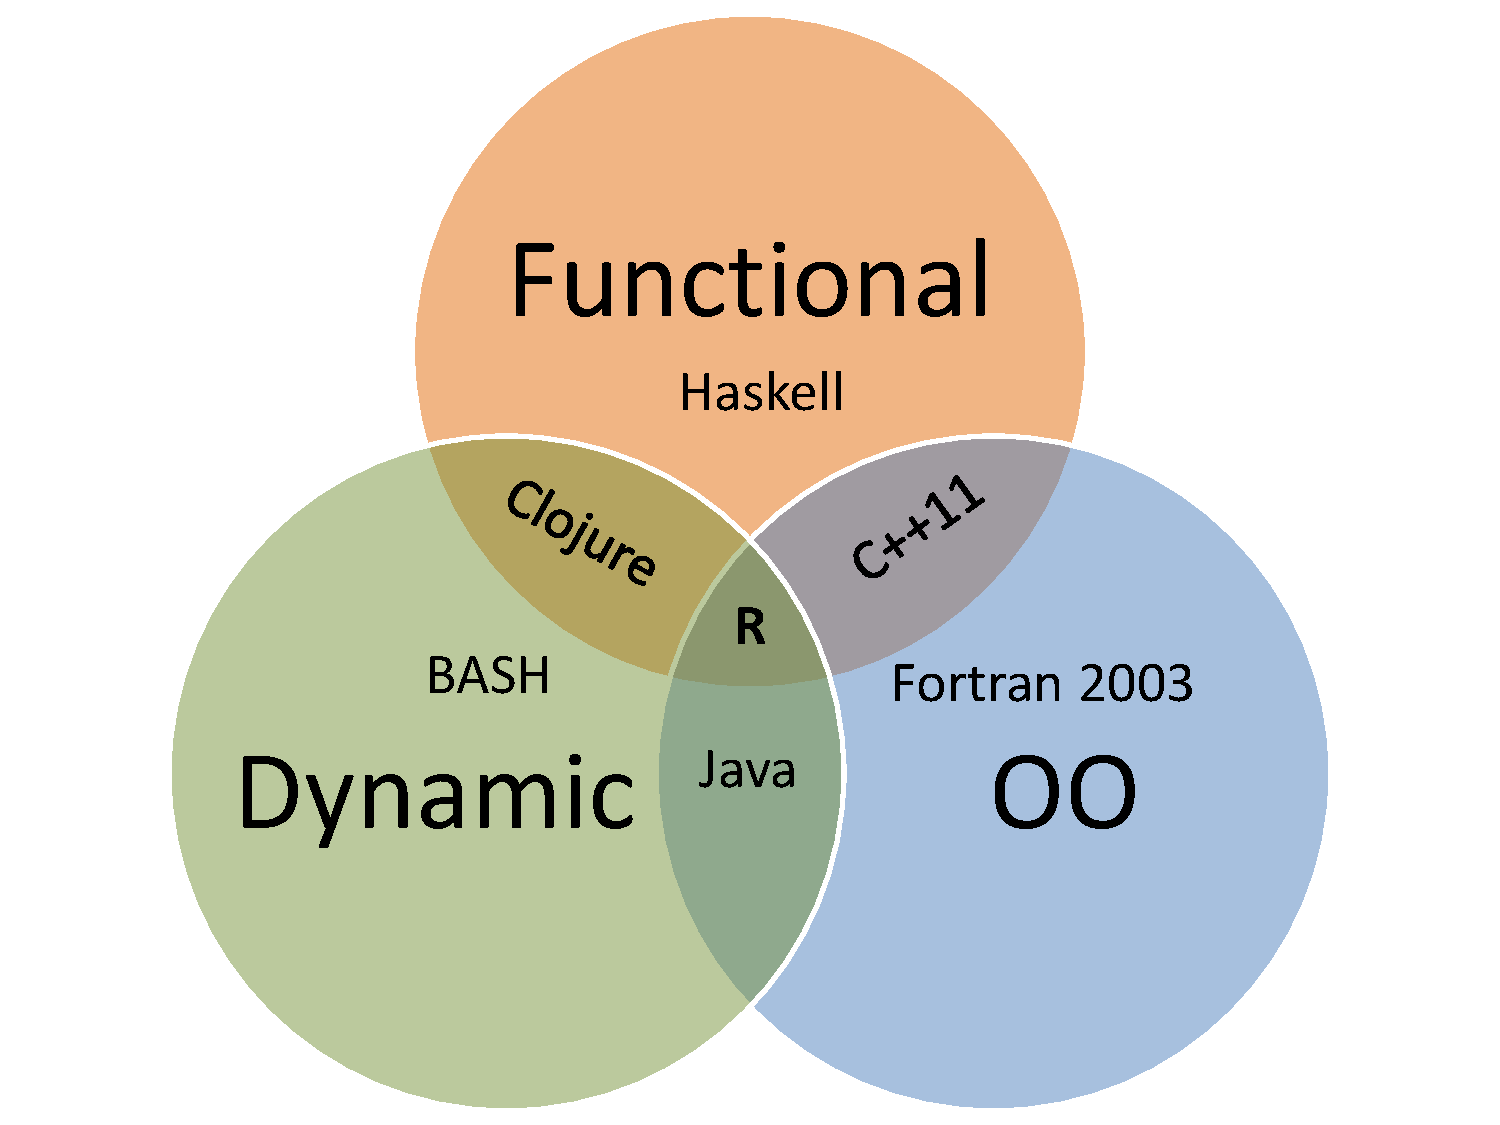
\includegraphics[scale=.35]{../common/pics/languages}
  \end{center}
  \end{block}
\end{frame}

\begin{frame}
  \begin{block}{Data Types}\pause
  \begin{itemize}[<+-|alert@+>]
    \item Storage:  logical, int, double, double complex, character
    \item Structures:  vector, matrix, array, list, dataframe
    \item Caveats:  (Logical) \code{TRUE}, \code{FALSE}, \code{NA}
  \end{itemize}
  For the remainder of the tutorial, we will restrict ourselves to real number 
matrix computations.
\end{block}
\end{frame}




\subsection{Syntax for Data Science}


\begin{frame}[fragile]
\begin{block}{High Level Syntax}\pause
\begin{lstlisting}
x <- matrix(rnorm(30), nrow=10)
x <- x[-1, 2:5]
x <- log(abs(x) + 1)
xtx <- t(x) %*% x
ans <- svd(solve(xtx))
\end{lstlisting}
\end{block}
\end{frame}


\begin{frame}
  \begin{block}{More than just a Matlab clone\dots}\pause
  \begin{itemize}[<+-|alert@+>]
    \item Data science (machine learning, statistics, data mining, \dots) is 
mostly matrix algebra.  \\[.2cm]
     So what about Matlab/Python/Julia/\dots ?
    \item Depends on your ``religion'' 
    \item As a \emph{data analysis} package, R is king.
  \end{itemize}
\end{block}
\end{frame}



\begin{frame}[fragile]
\begin{block}{High Level Syntax \emph{for Data}}\pause
\begin{lstlisting}
pca <- prcomp(x, retx=TRUE, scale=TRUE)
prop_var <- cumsum(pca$sdev)/sum(pca$sdev)
i <- min(which(prop_var > 0.9)) - 1

y <- pca$x[, 1:i]
\end{lstlisting}
\end{block}
\end{frame}

















\section{Parallel Hardware and R}

\hidenum
\begin{frame}[noframenumbering]
\frametitle{Contents}
 \tableofcontents[currentsection,hideothersubsections,sectionstyle=show/hide]
\end{frame}
\shownum

\subsection{Parallel Hardware}

% \begin{frame}
% \begin{block}{A}
%   
% \end{block}
% \end{frame}


\begin{frame}
\begin{block}{Three Basic Flavors of Hardware}
    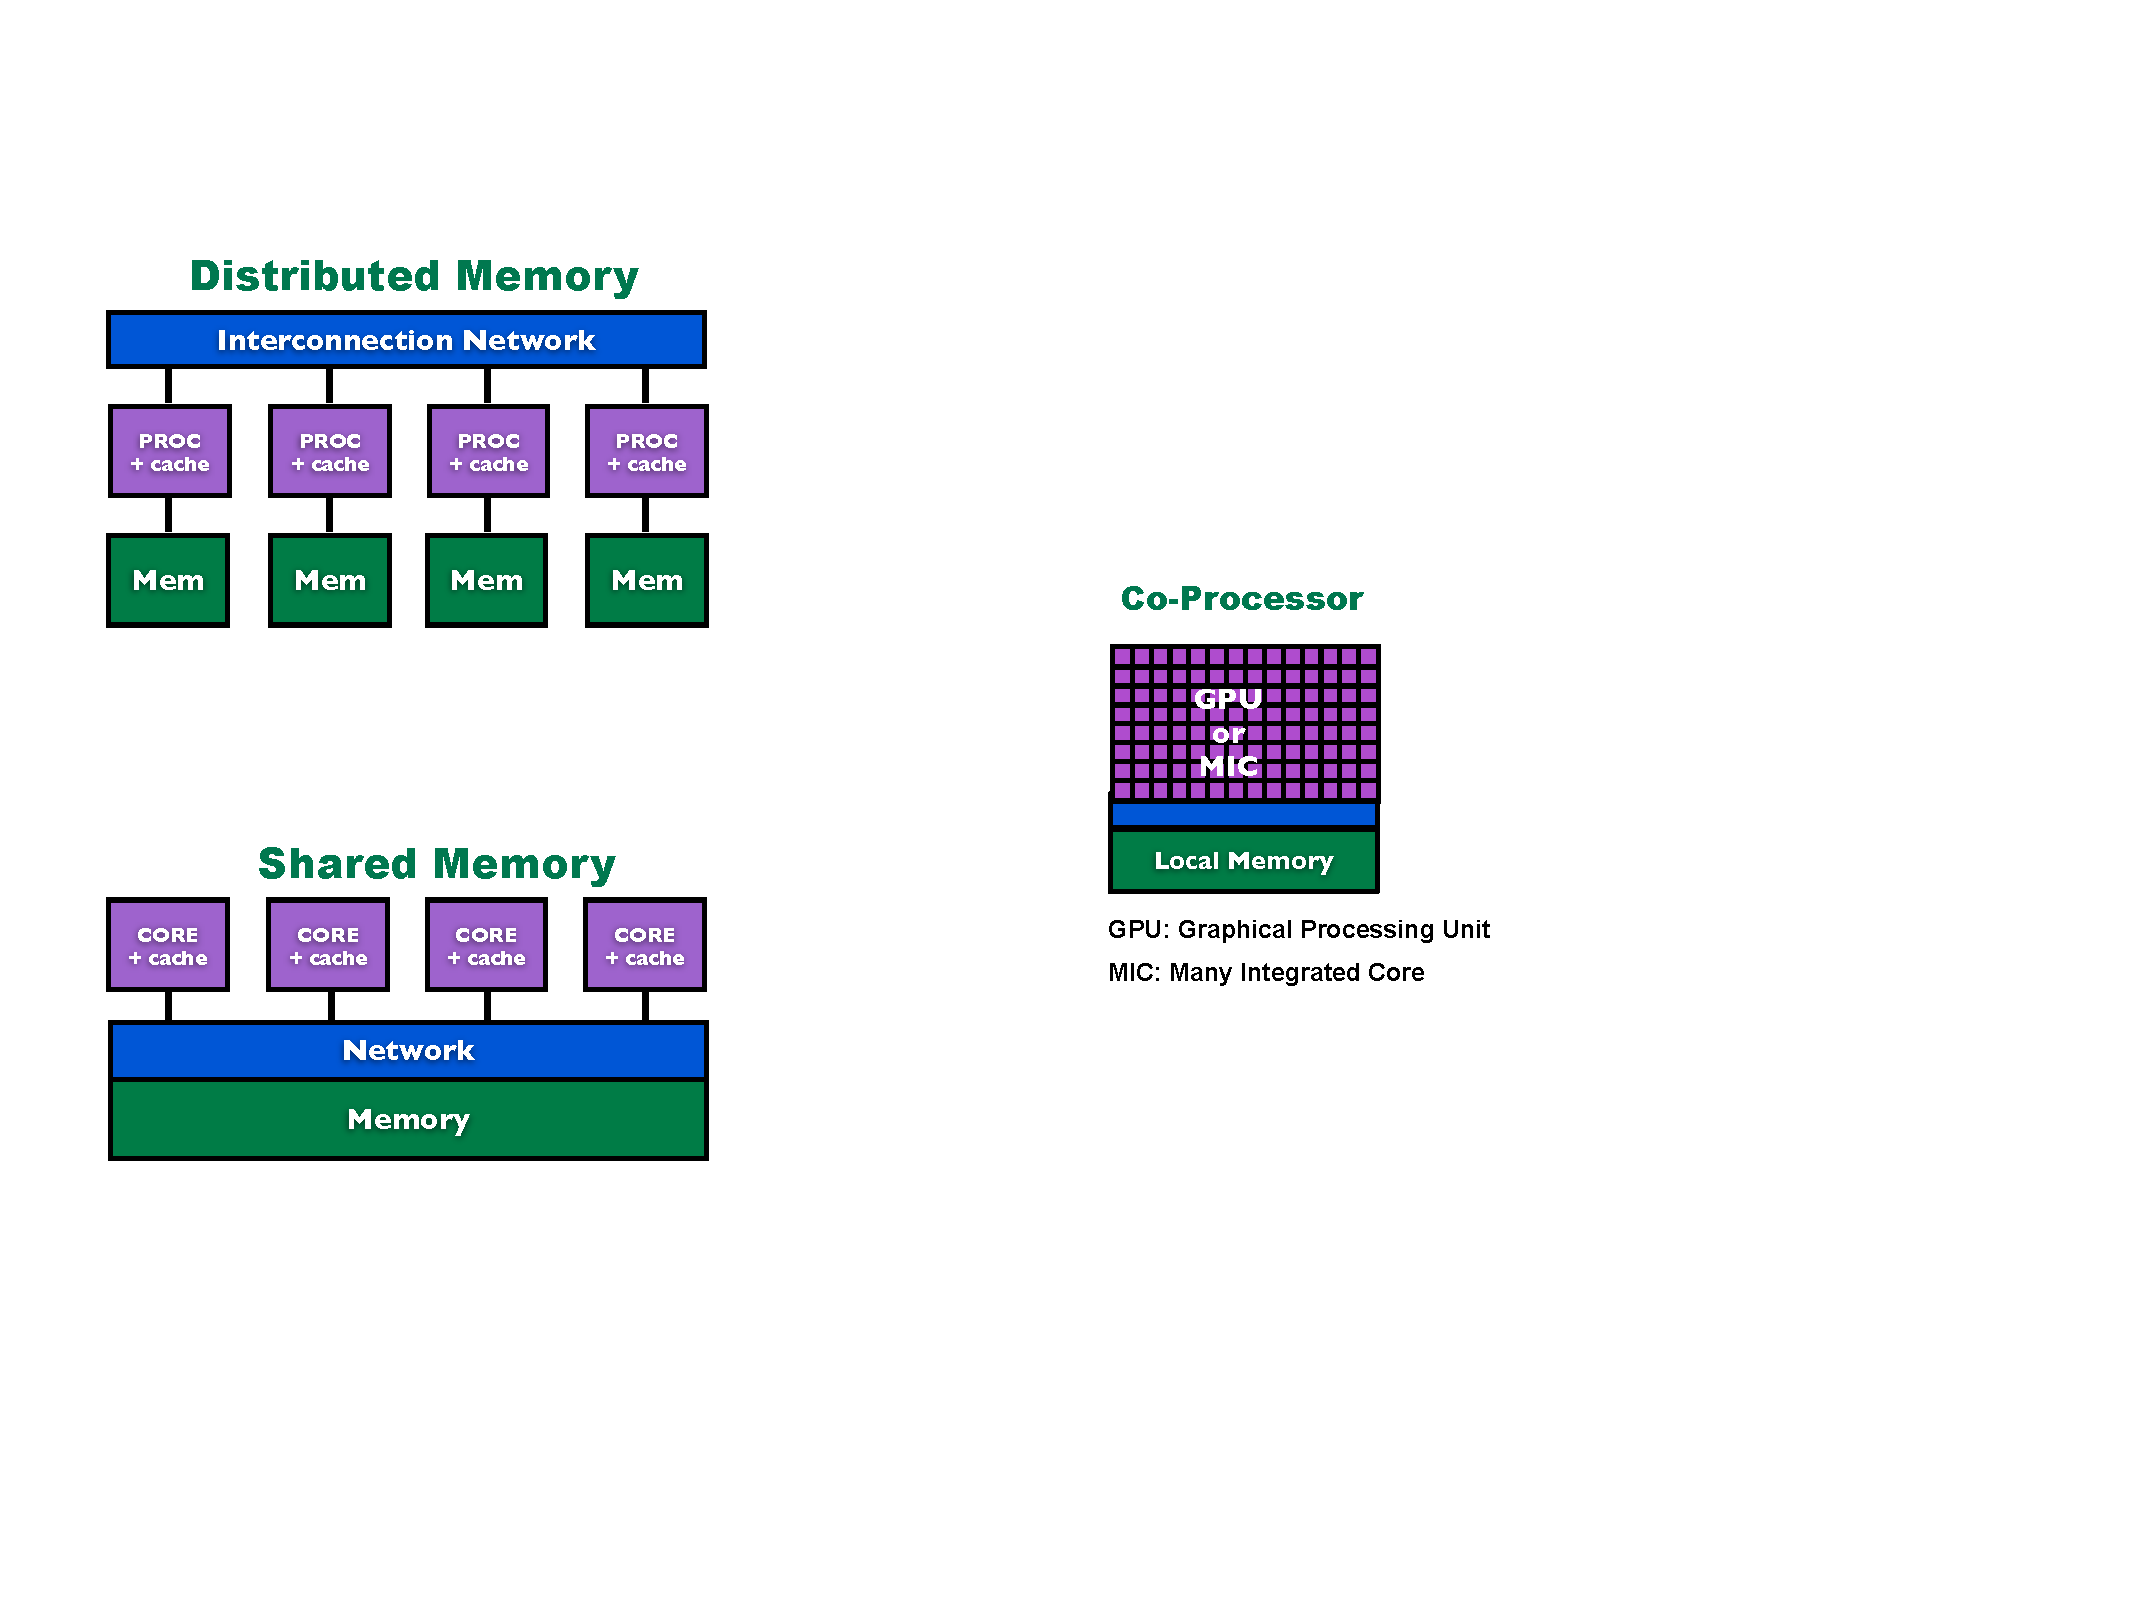
\includegraphics[width=0.95\textwidth]{../common/pics/ParallelHardware1.pdf}
\end{block}
\end{frame}

\begin{frame}
\begin{block}{Your Laptop or Desktop}
    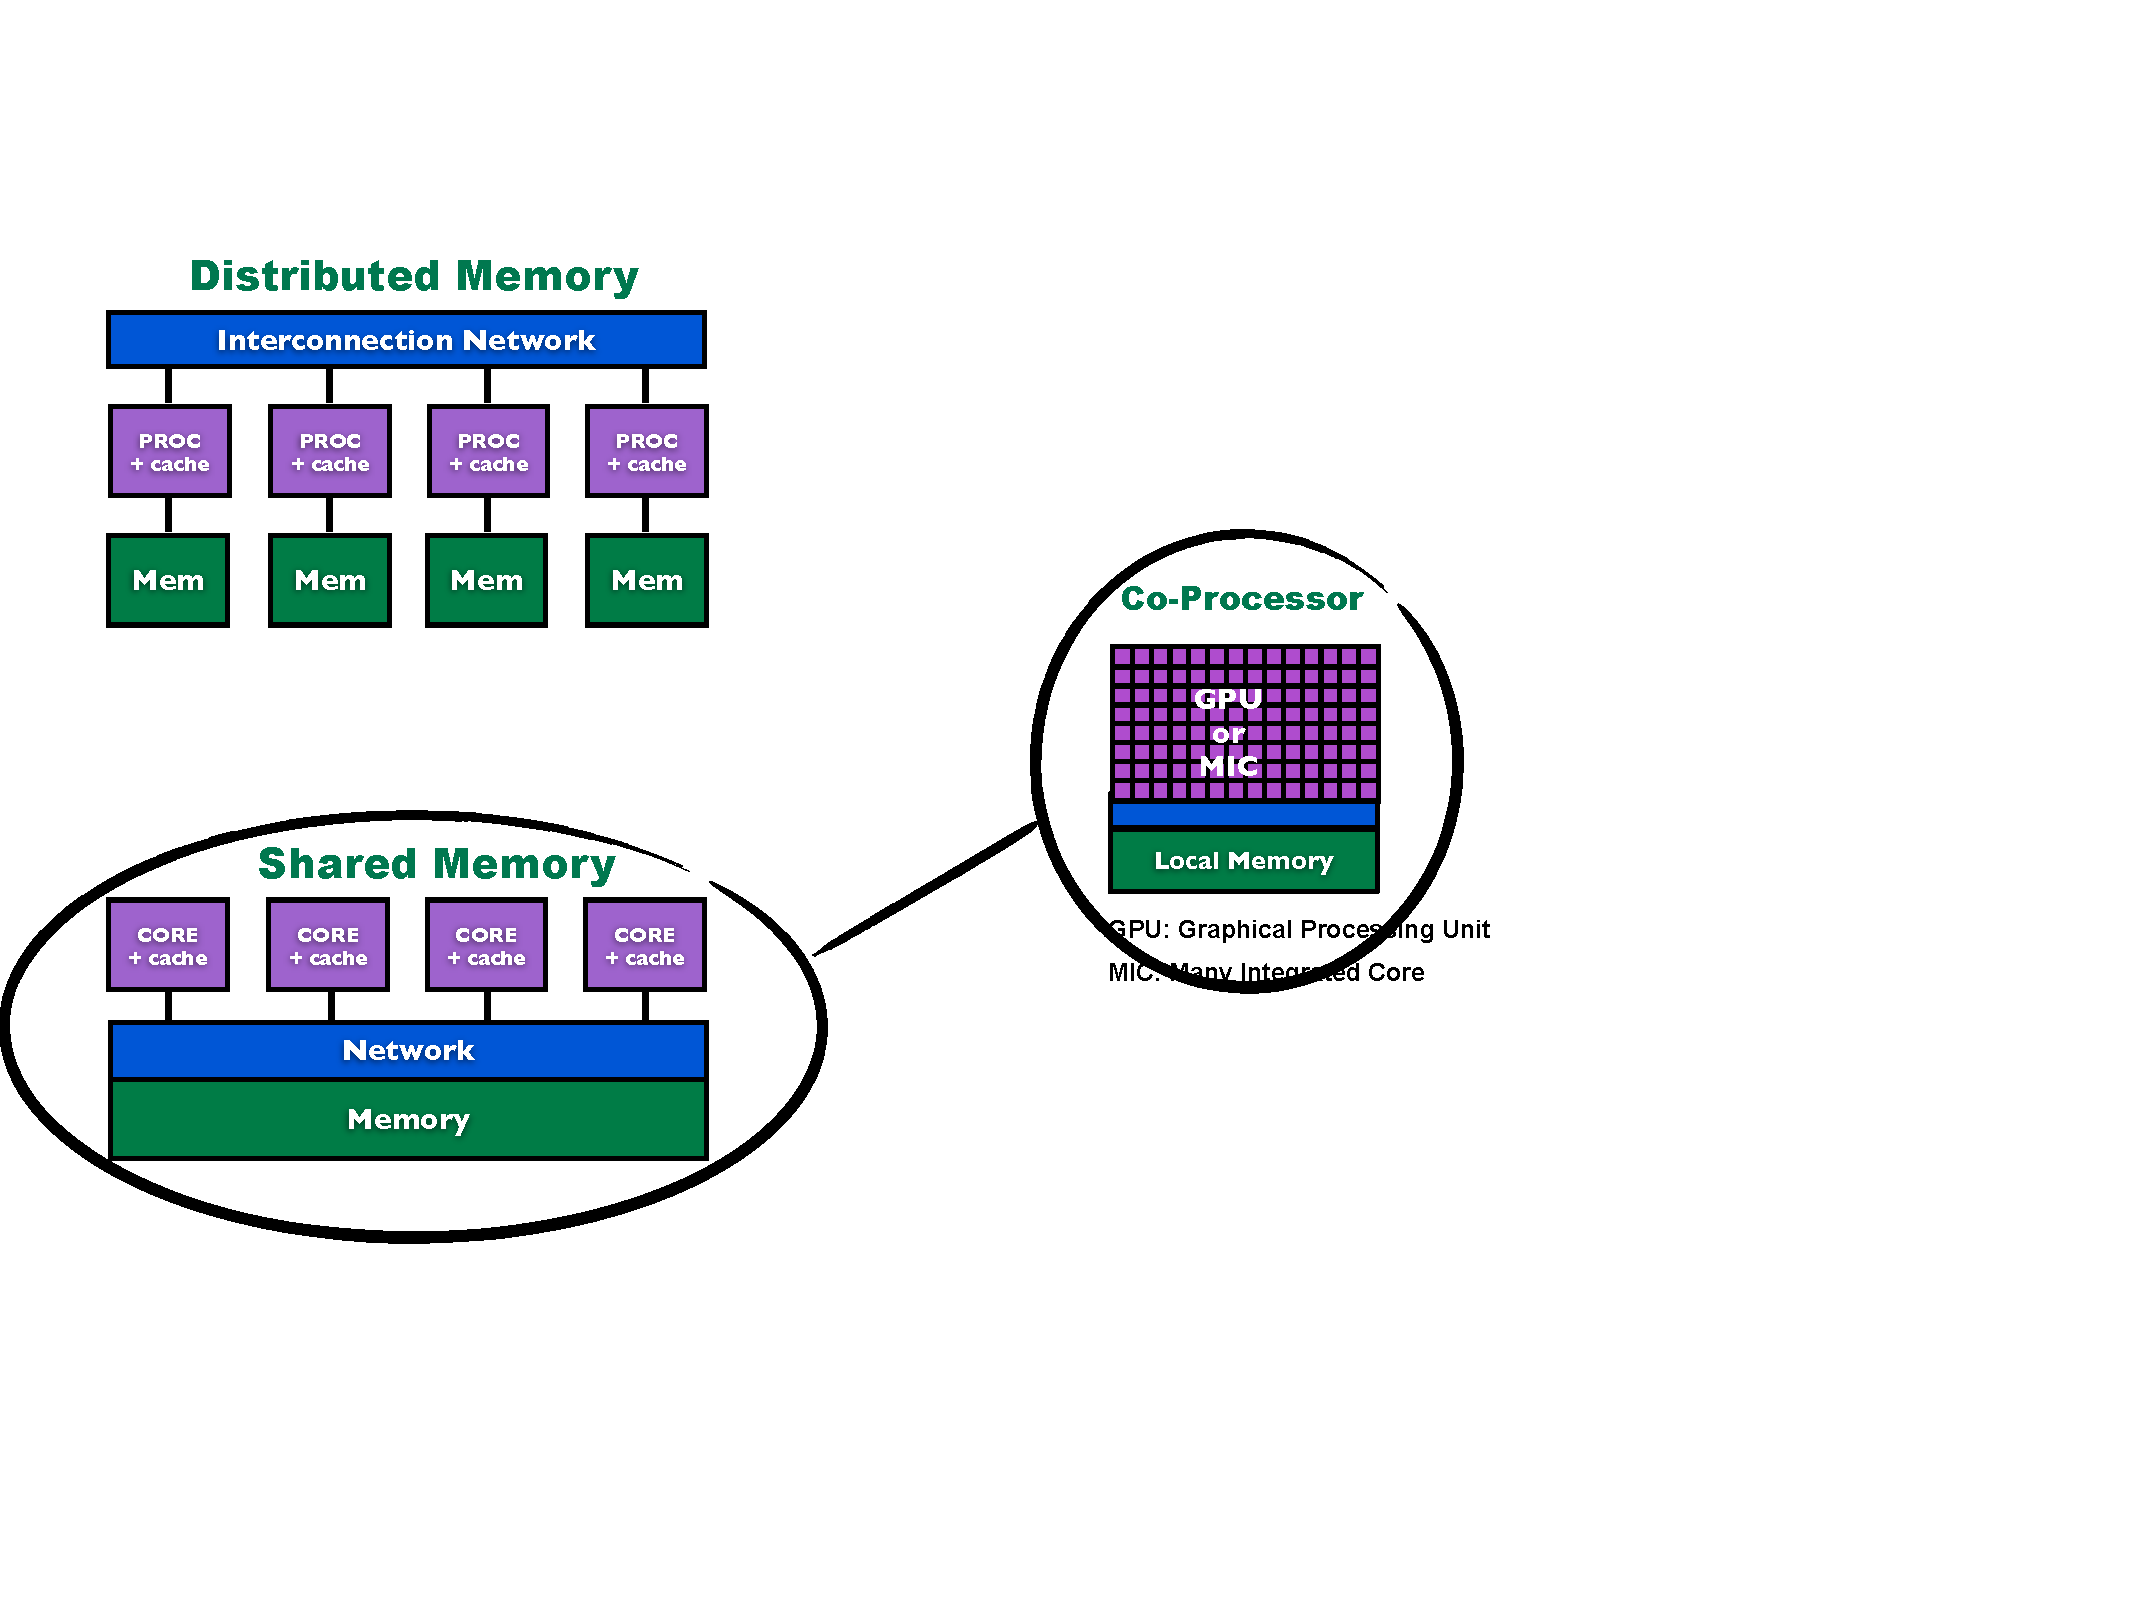
\includegraphics[width=0.95\textwidth]{../common/pics/ParallelHardware2.pdf}
\end{block}
\end{frame}

\begin{frame}
\begin{block}{A Server or Cluster}
    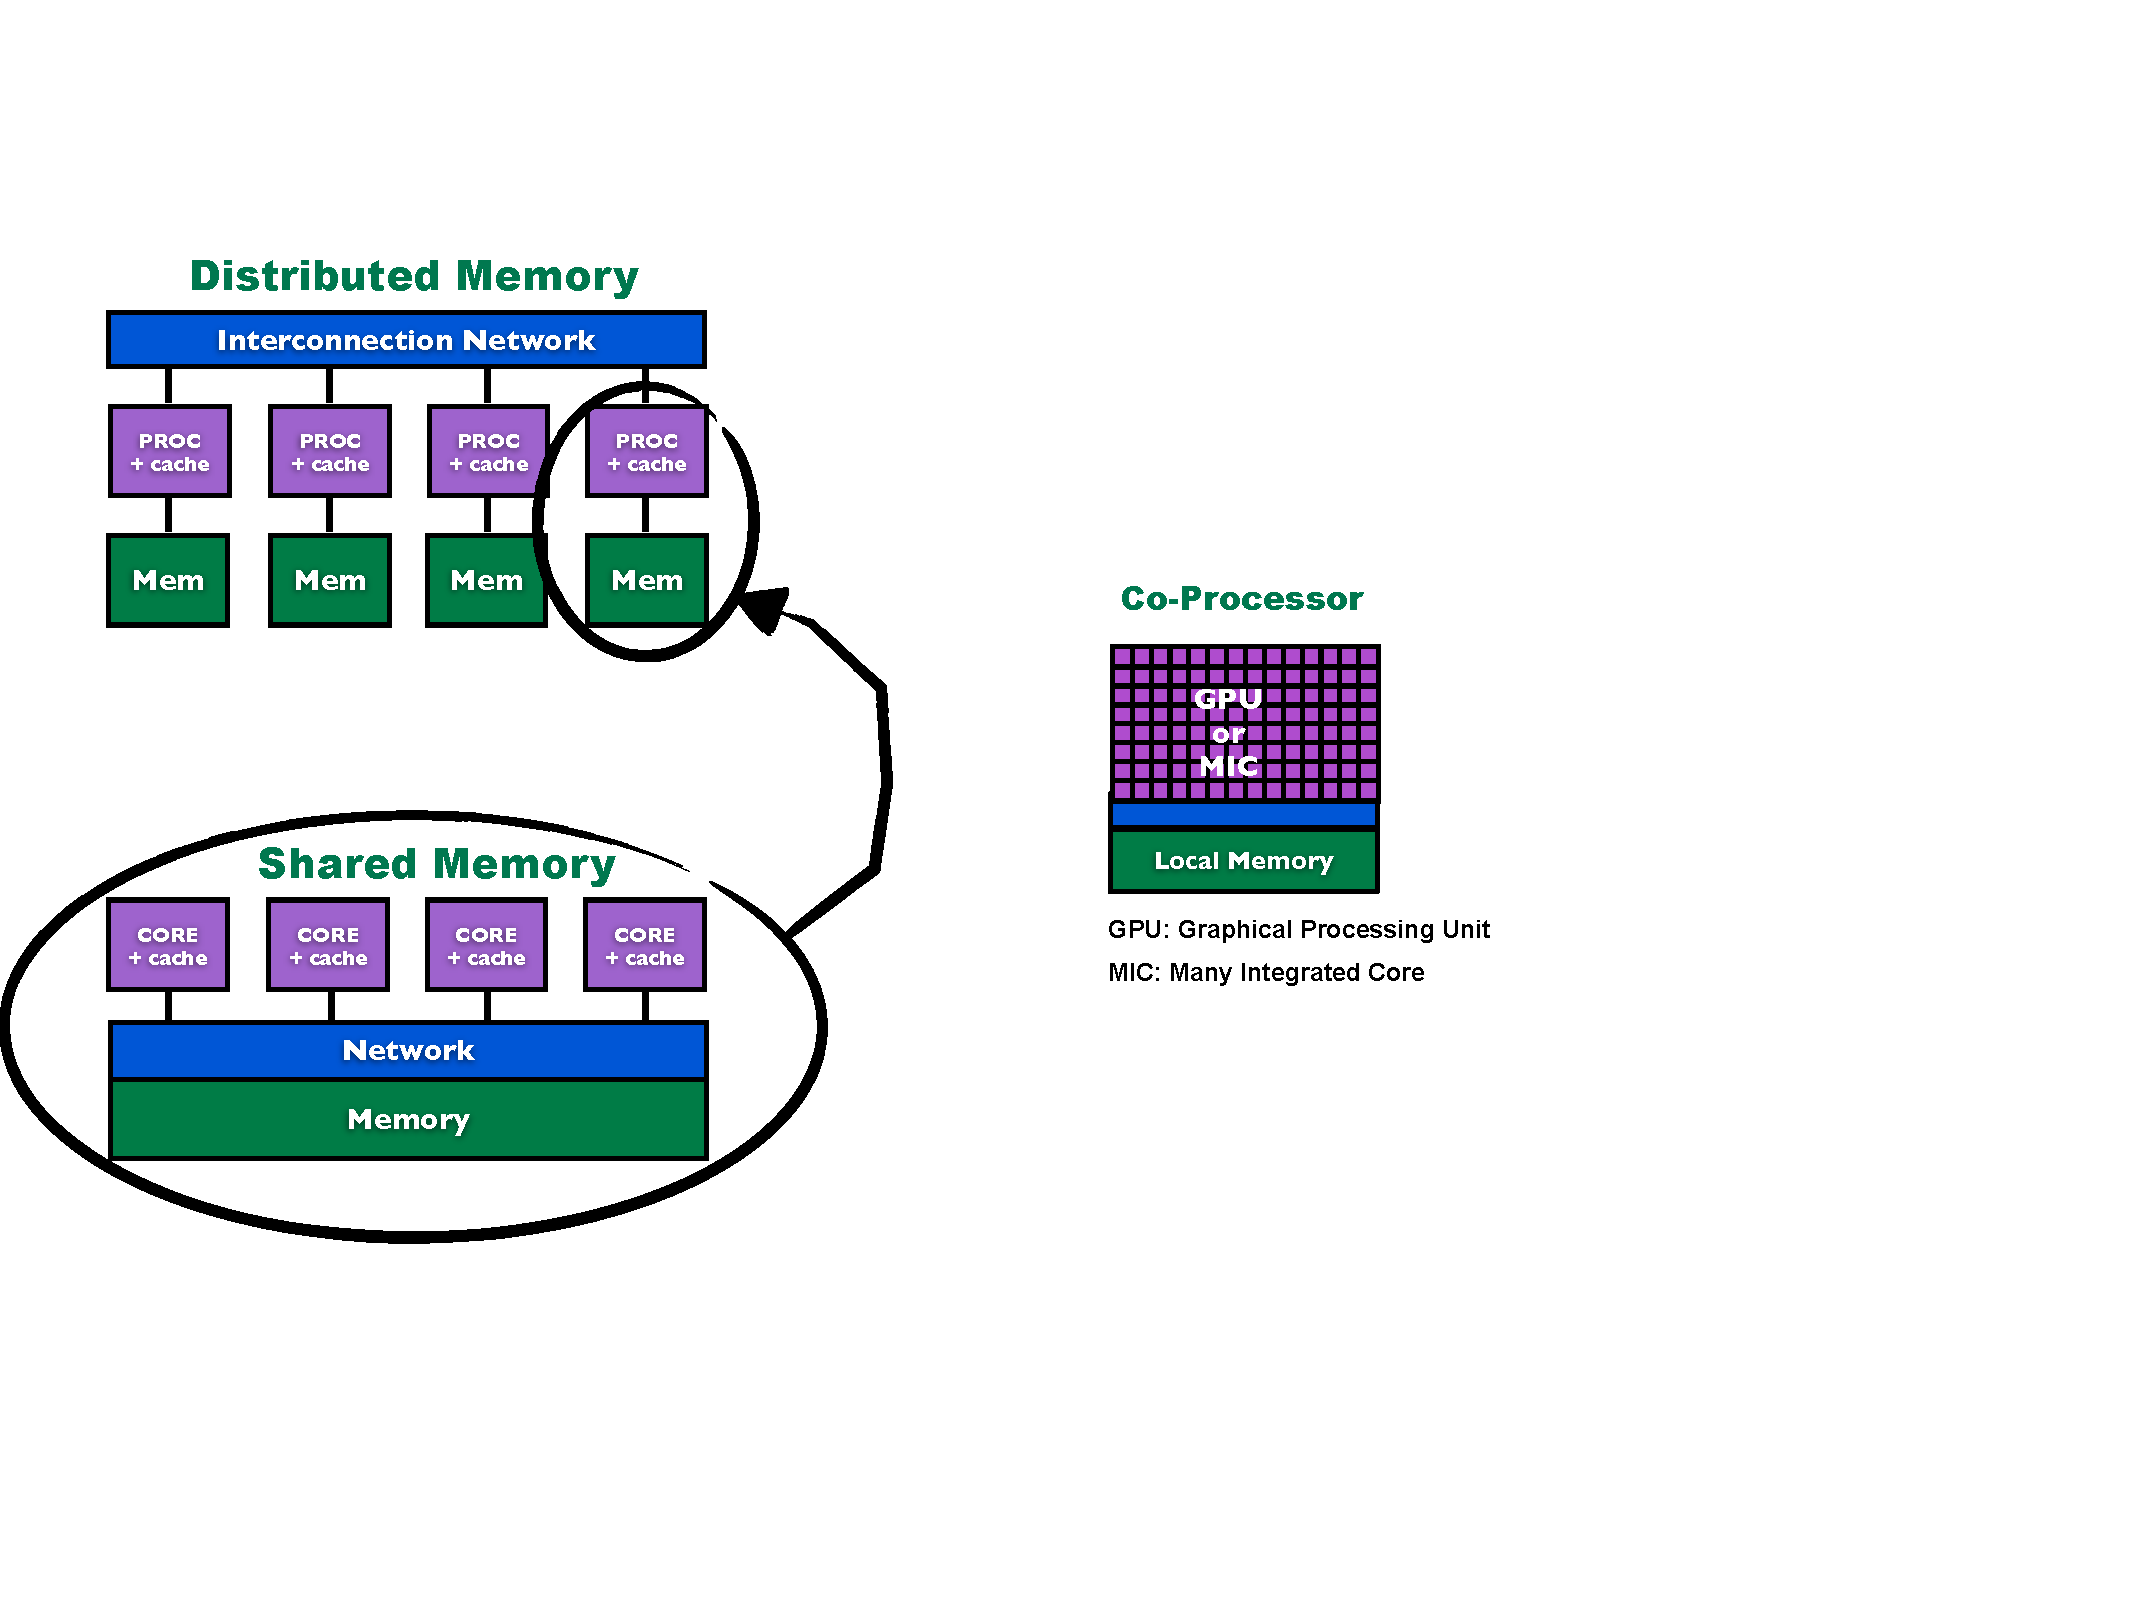
\includegraphics[width=0.95\textwidth]{../common/pics/ParallelHardware3.pdf}
\end{block}
\end{frame}

\begin{frame}
\begin{block}{Server to Supercomputer}
    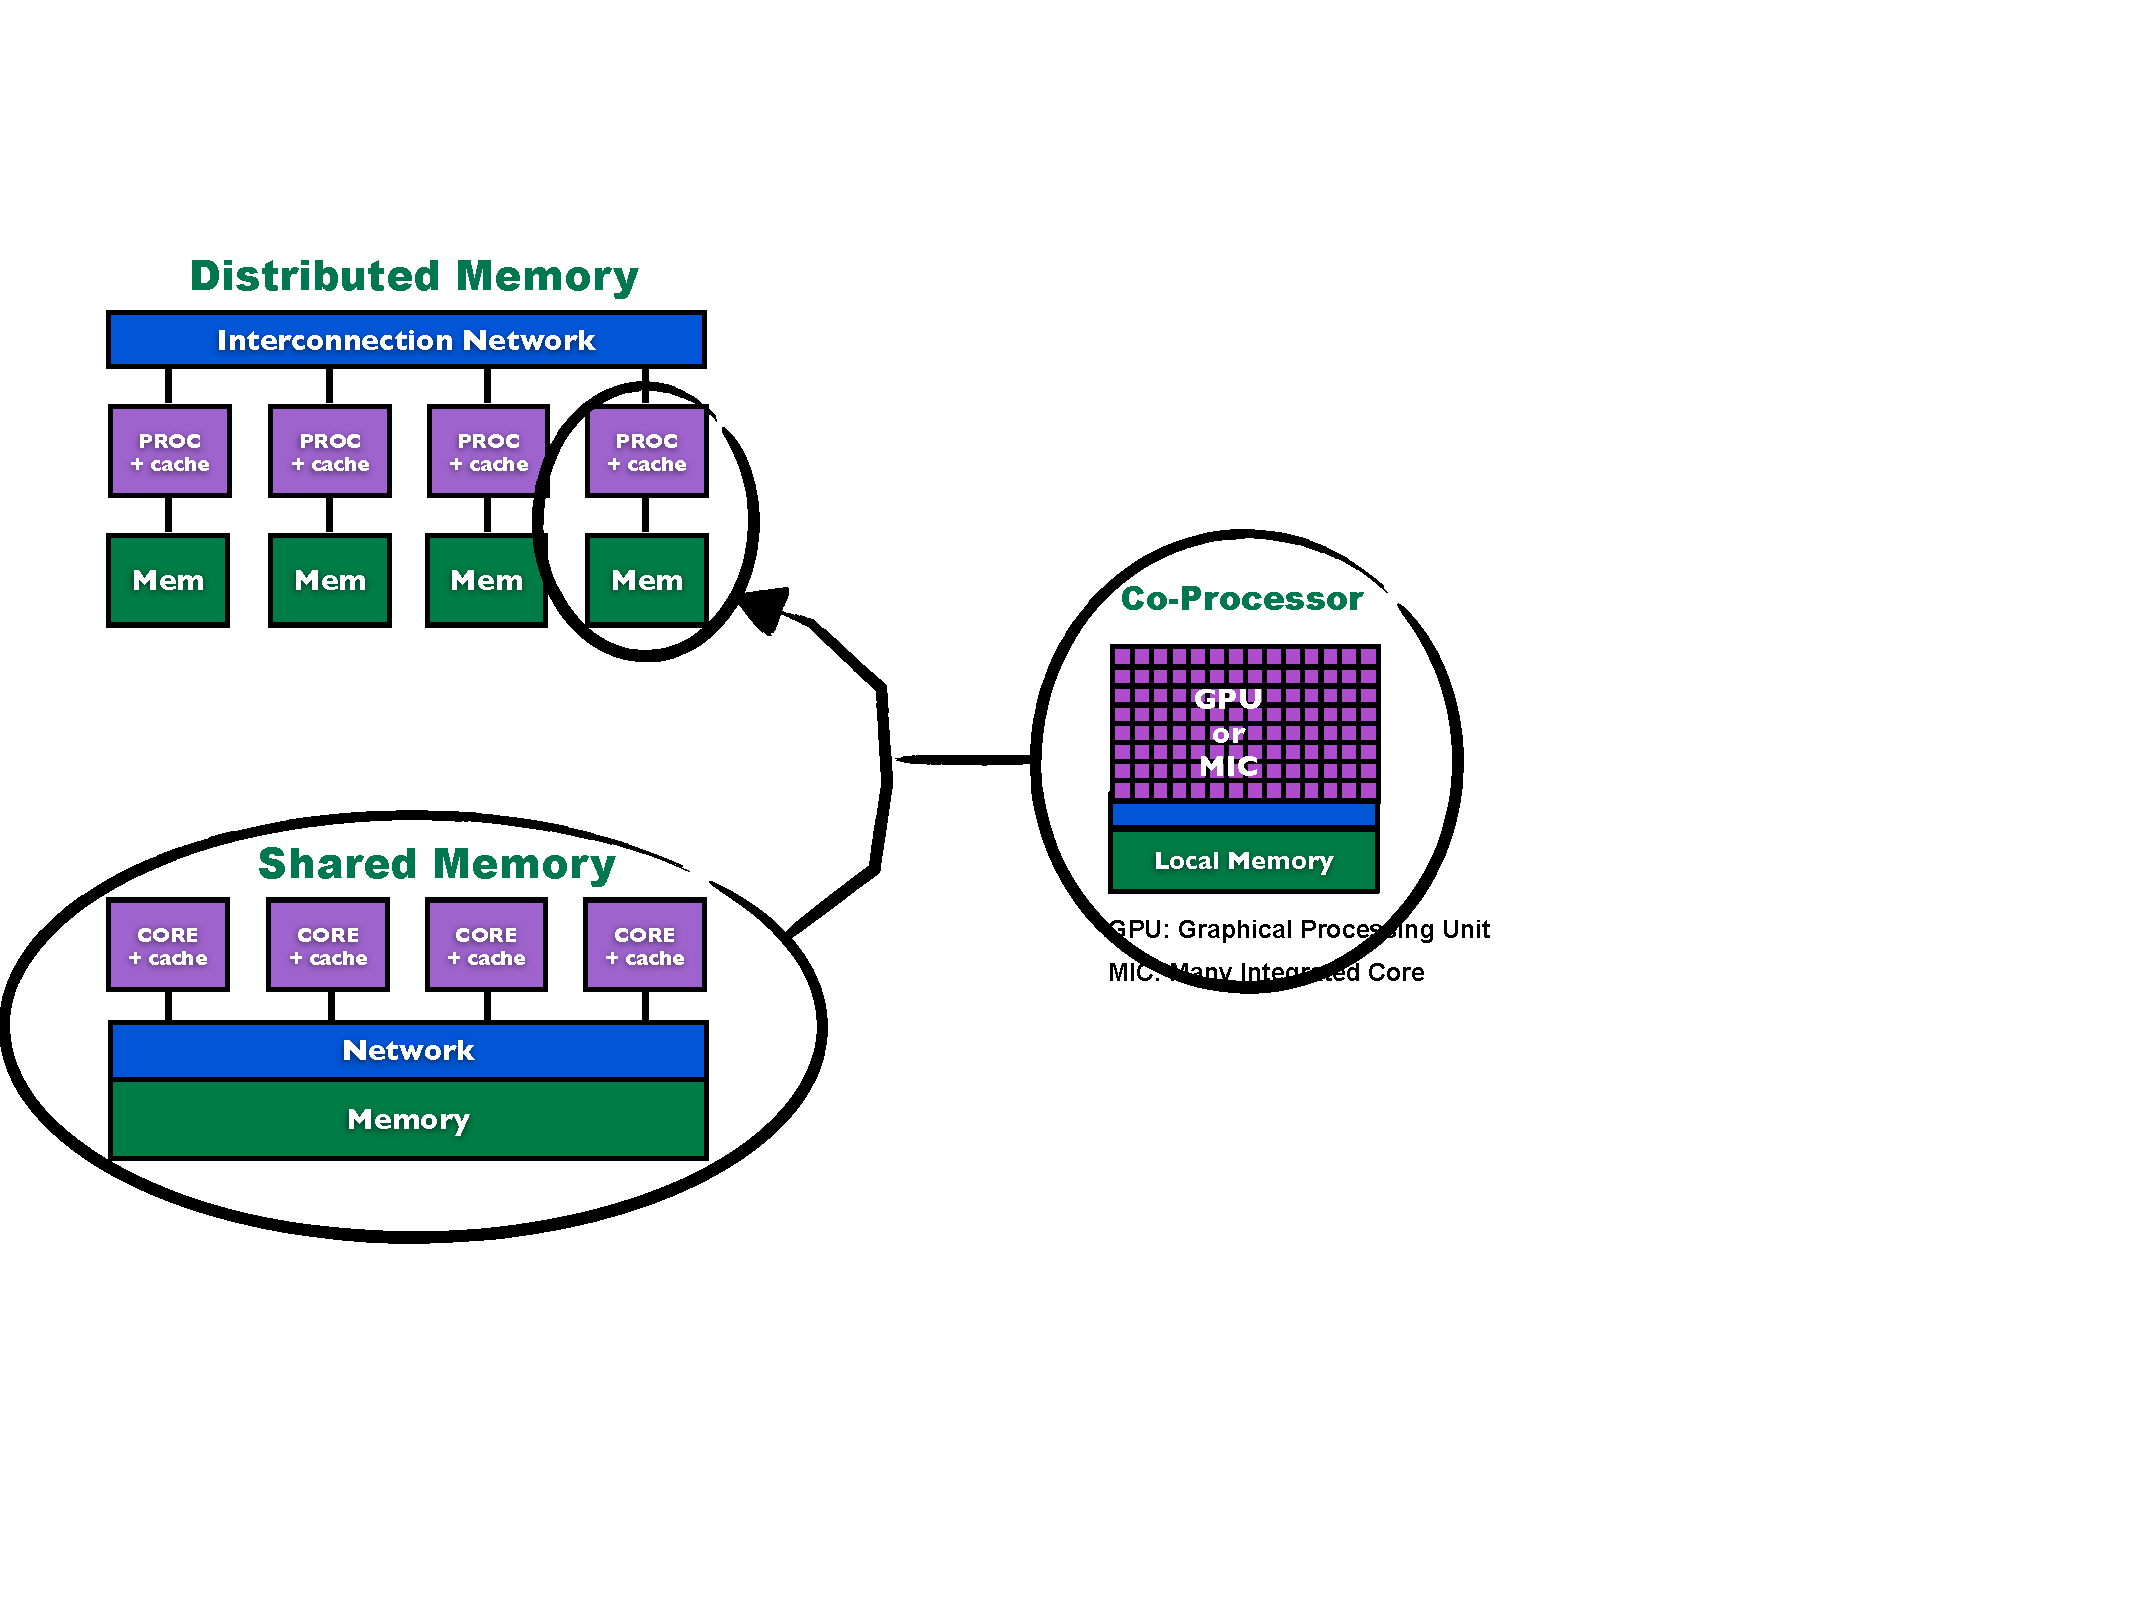
\includegraphics[width=0.95\textwidth]{../common/pics/ParallelHardware4.pdf}
\end{block}
\end{frame}

\begin{frame}
\begin{block}{Knowing the Right Words}
    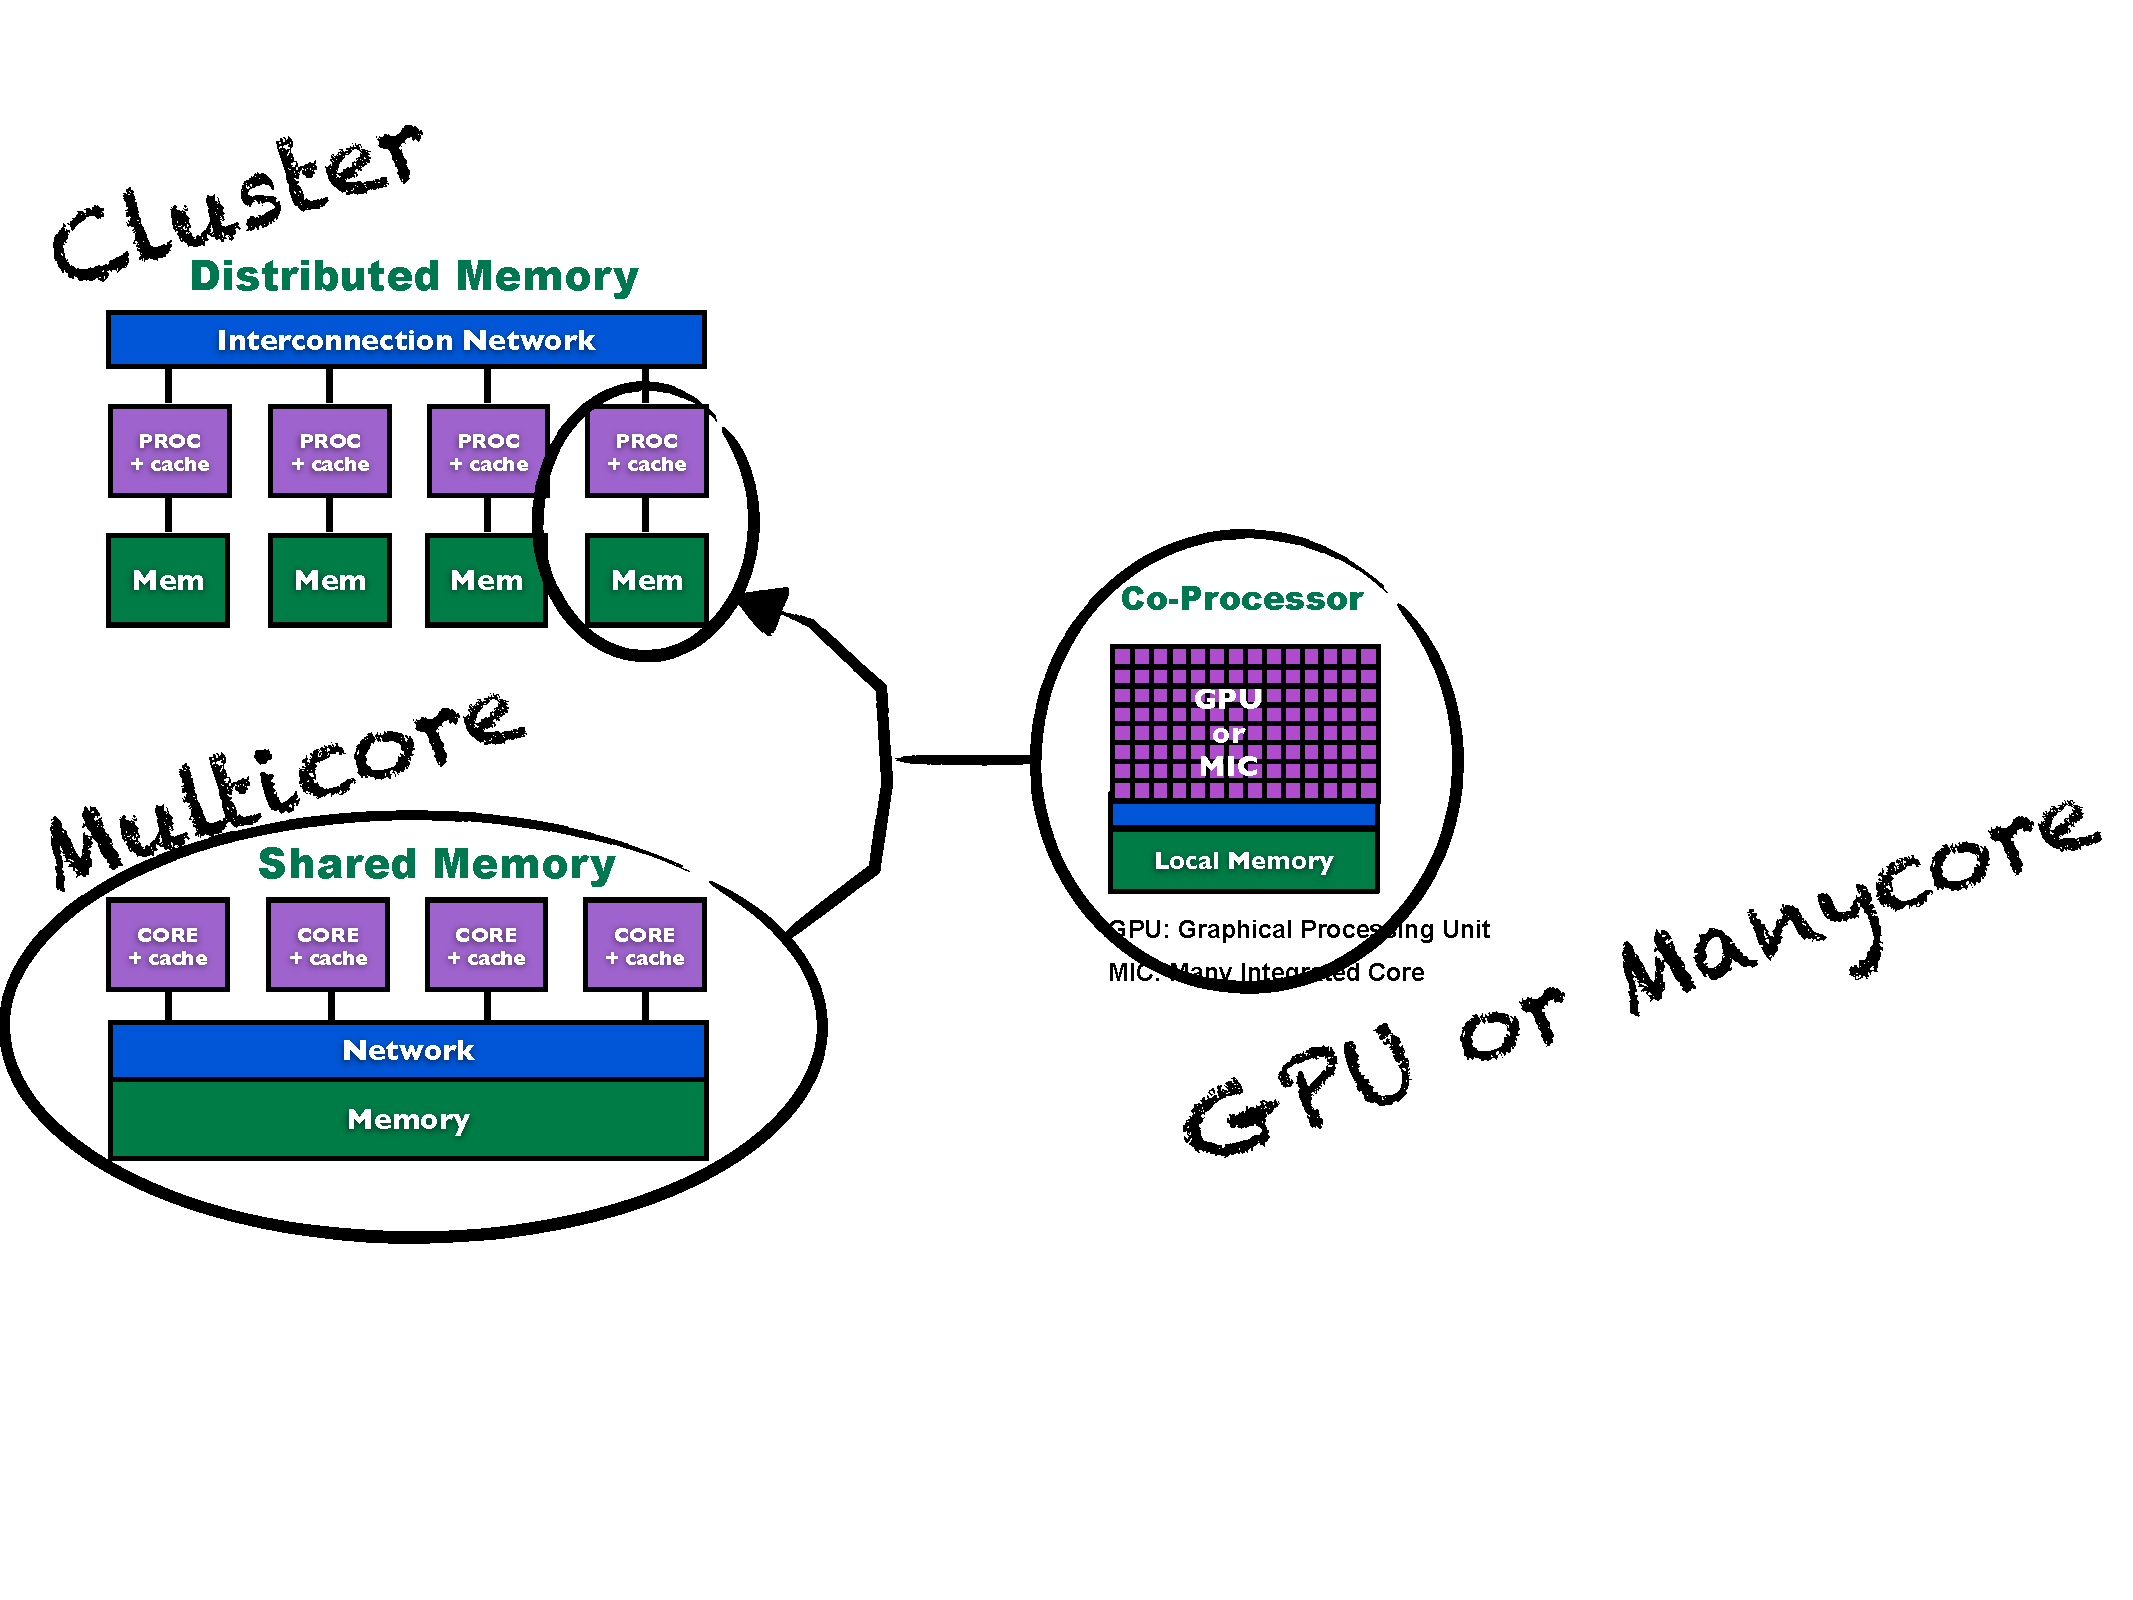
\includegraphics[width=0.95\textwidth]{../common/pics/ParallelHardware5.pdf}
\end{block}
\end{frame}

\begin{frame}
\begin{block}{``Native'' Programming Models and Tools}
    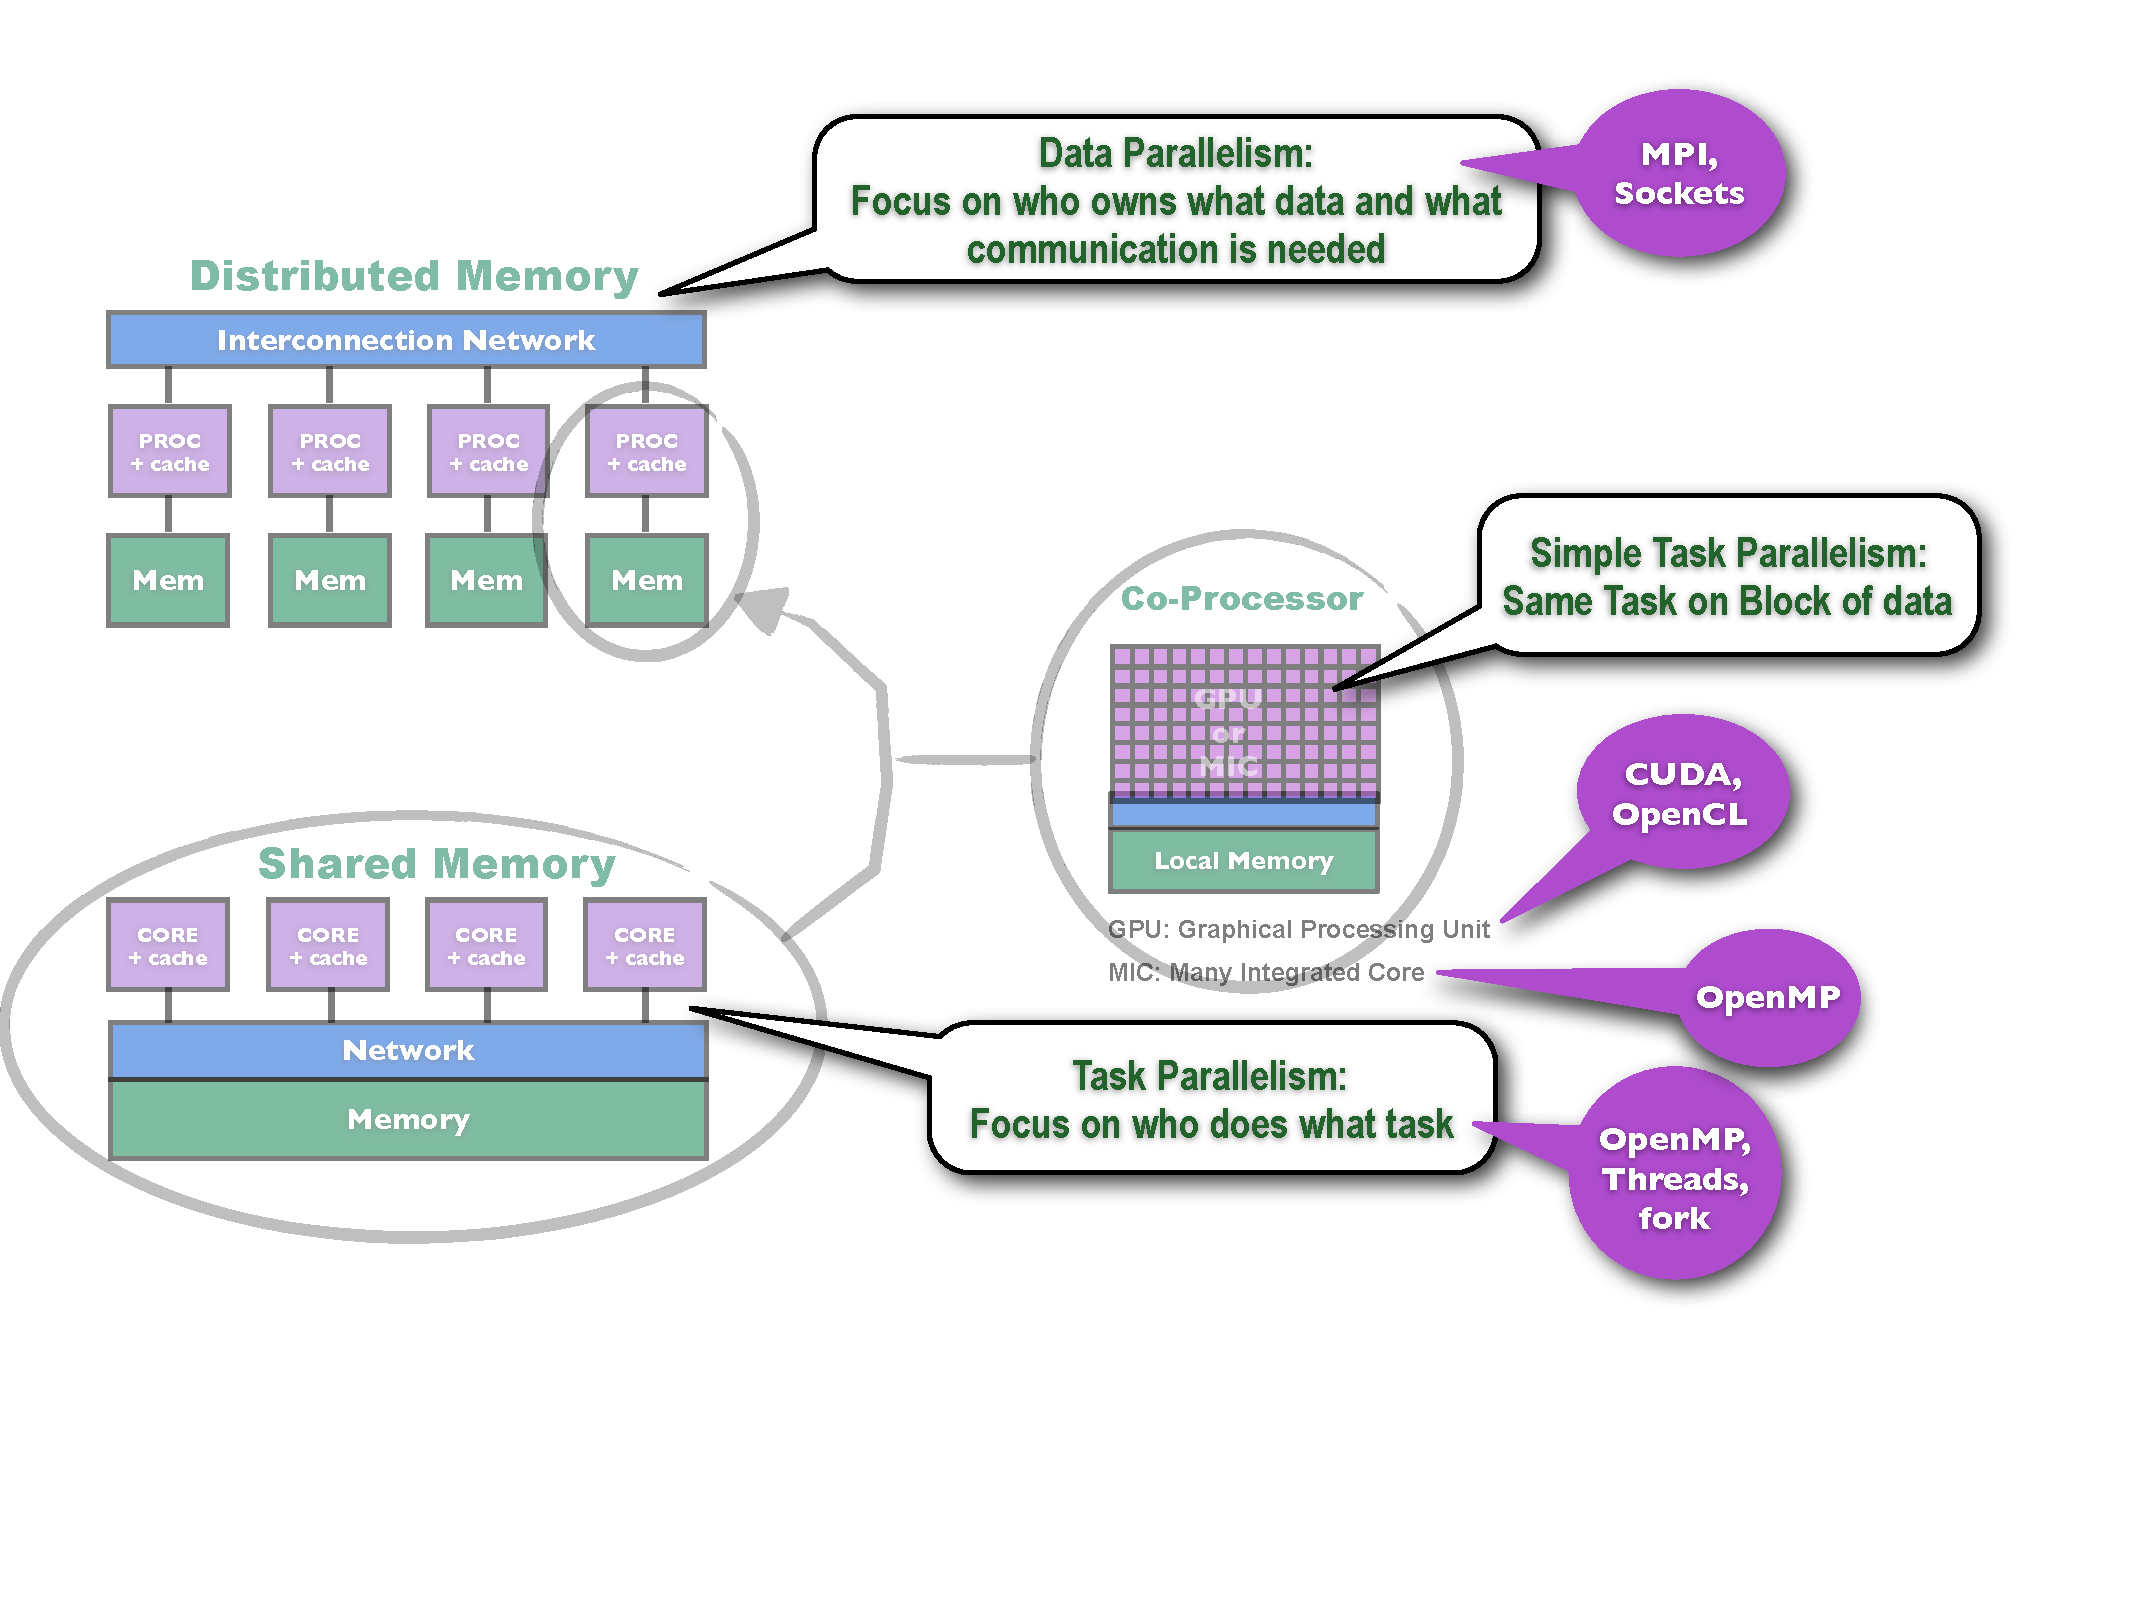
\includegraphics[width=0.95\textwidth]{../common/pics/ParallelHardware6.pdf}
\end{block}
\end{frame}

\subsection{R Interfaces to Parallel Hardware}

\begin{frame}
\begin{block}{R Interfaces to Native Tools}
    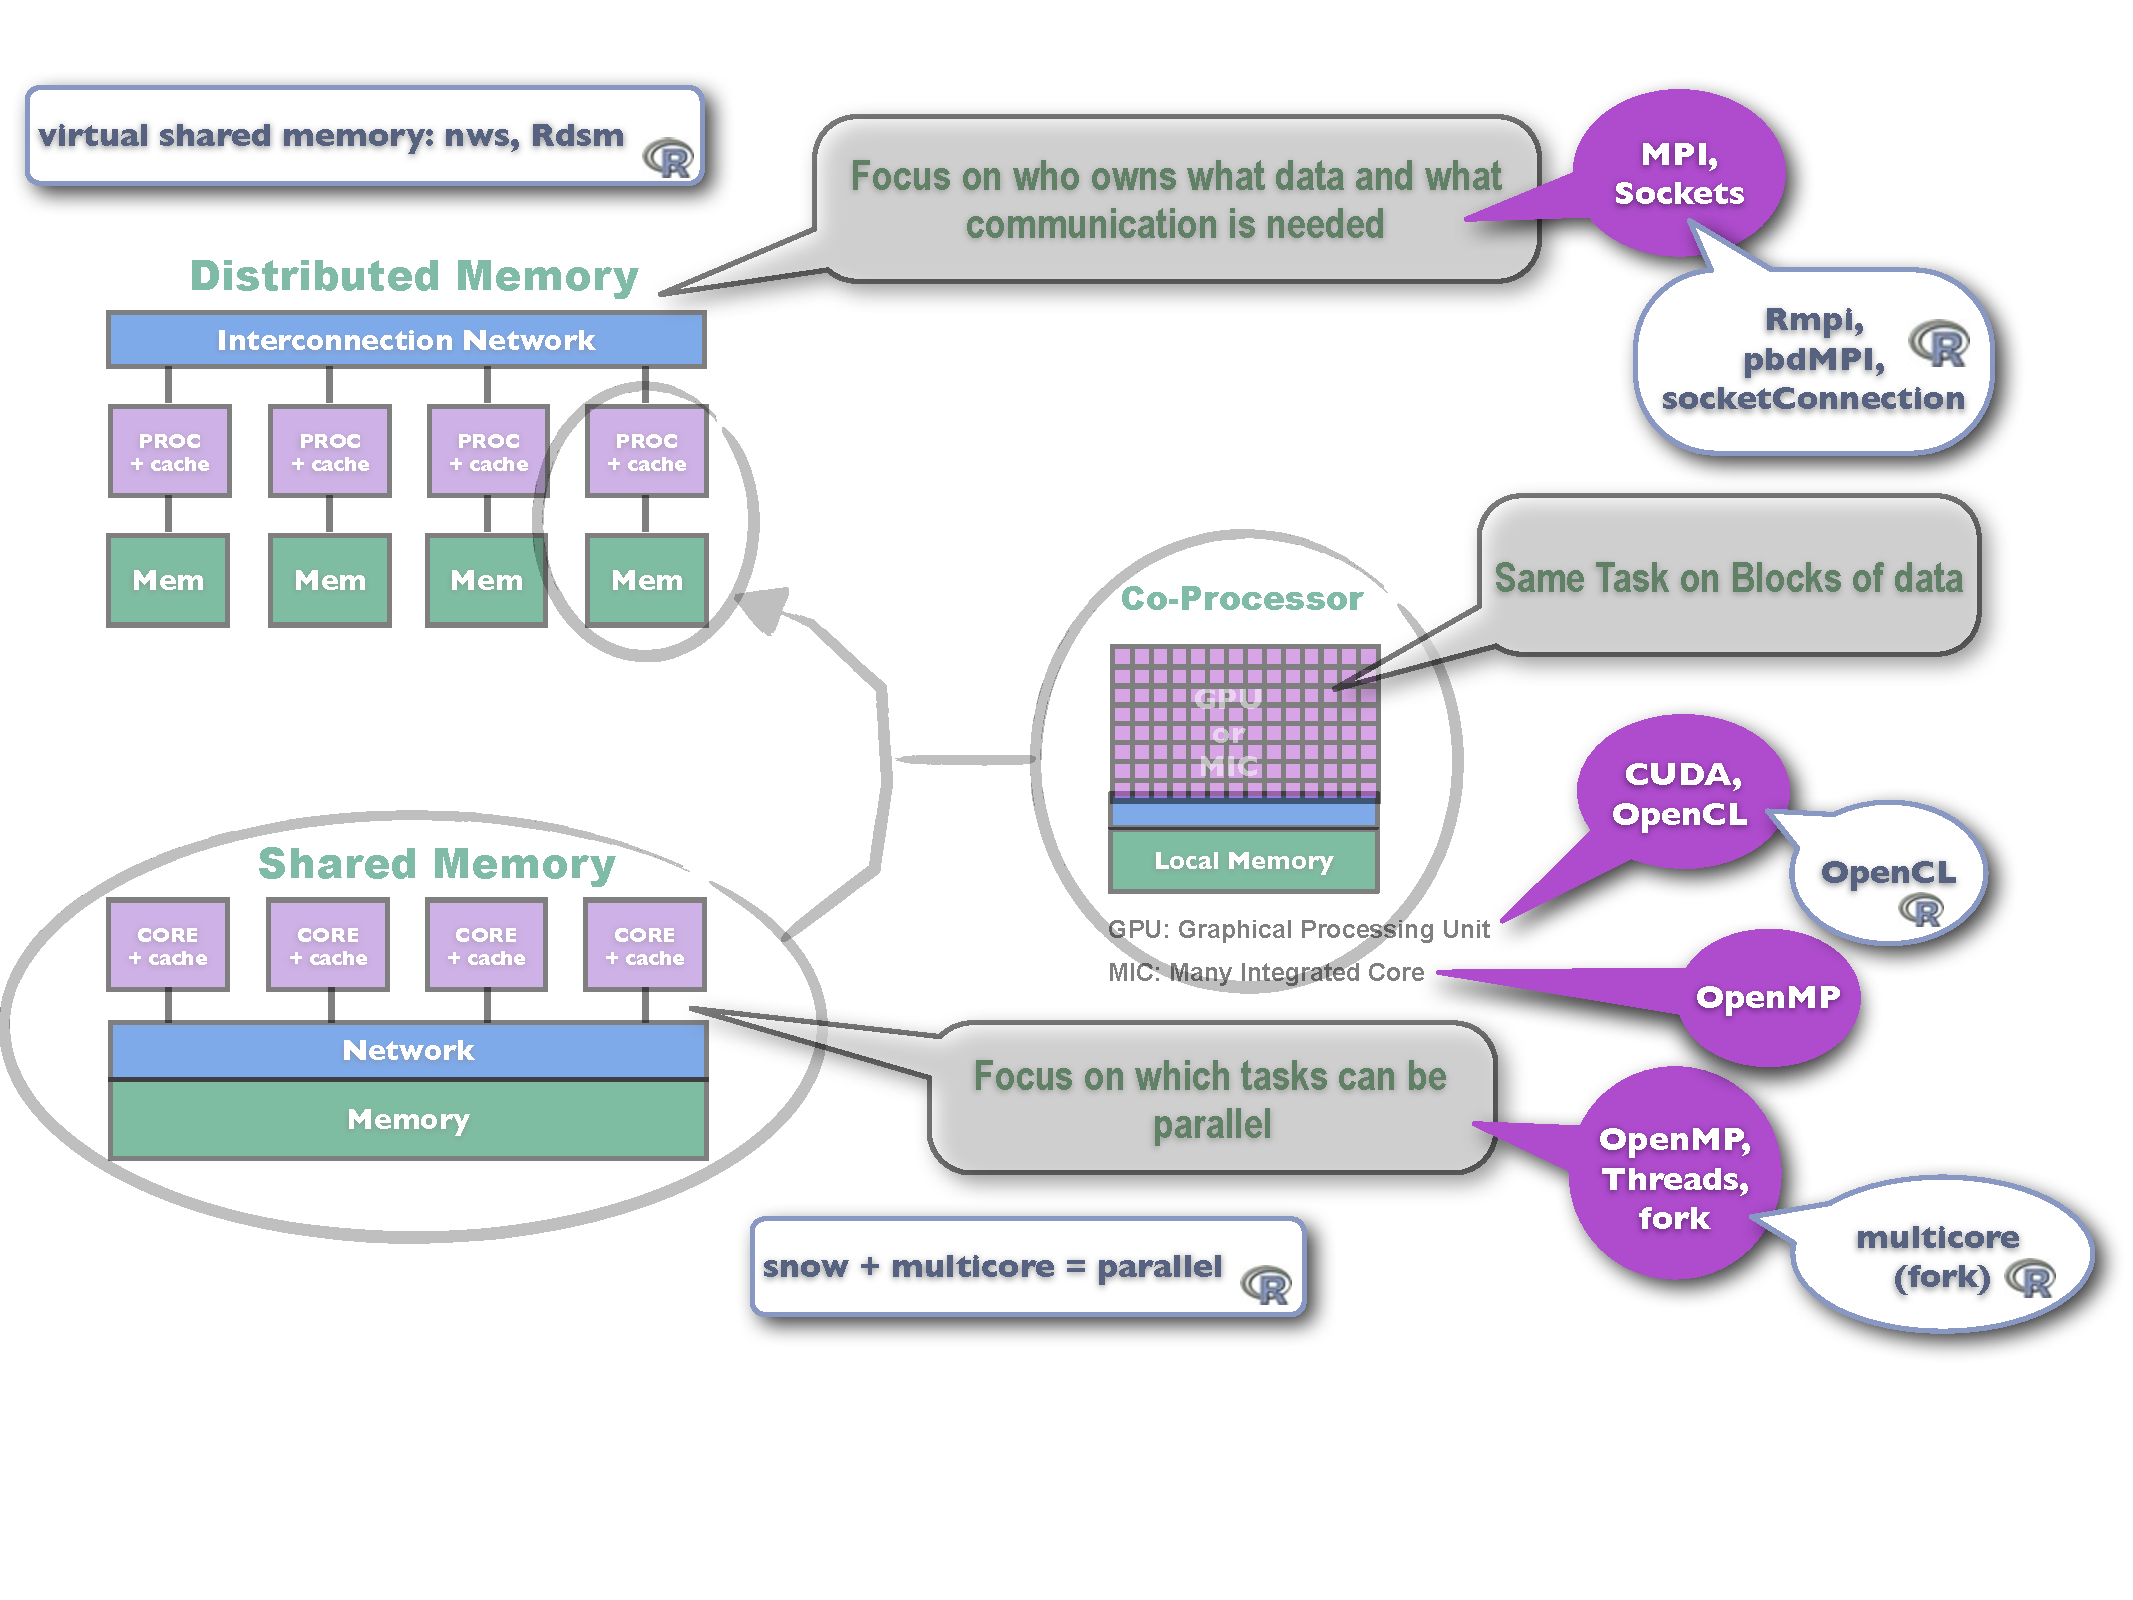
\includegraphics[width=0.95\textwidth]{../common/pics/ParallelHardware7.pdf}
\end{block}
\end{frame}

\begin{frame}
\begin{block}{30+ Years of Parallel Computing Research}
    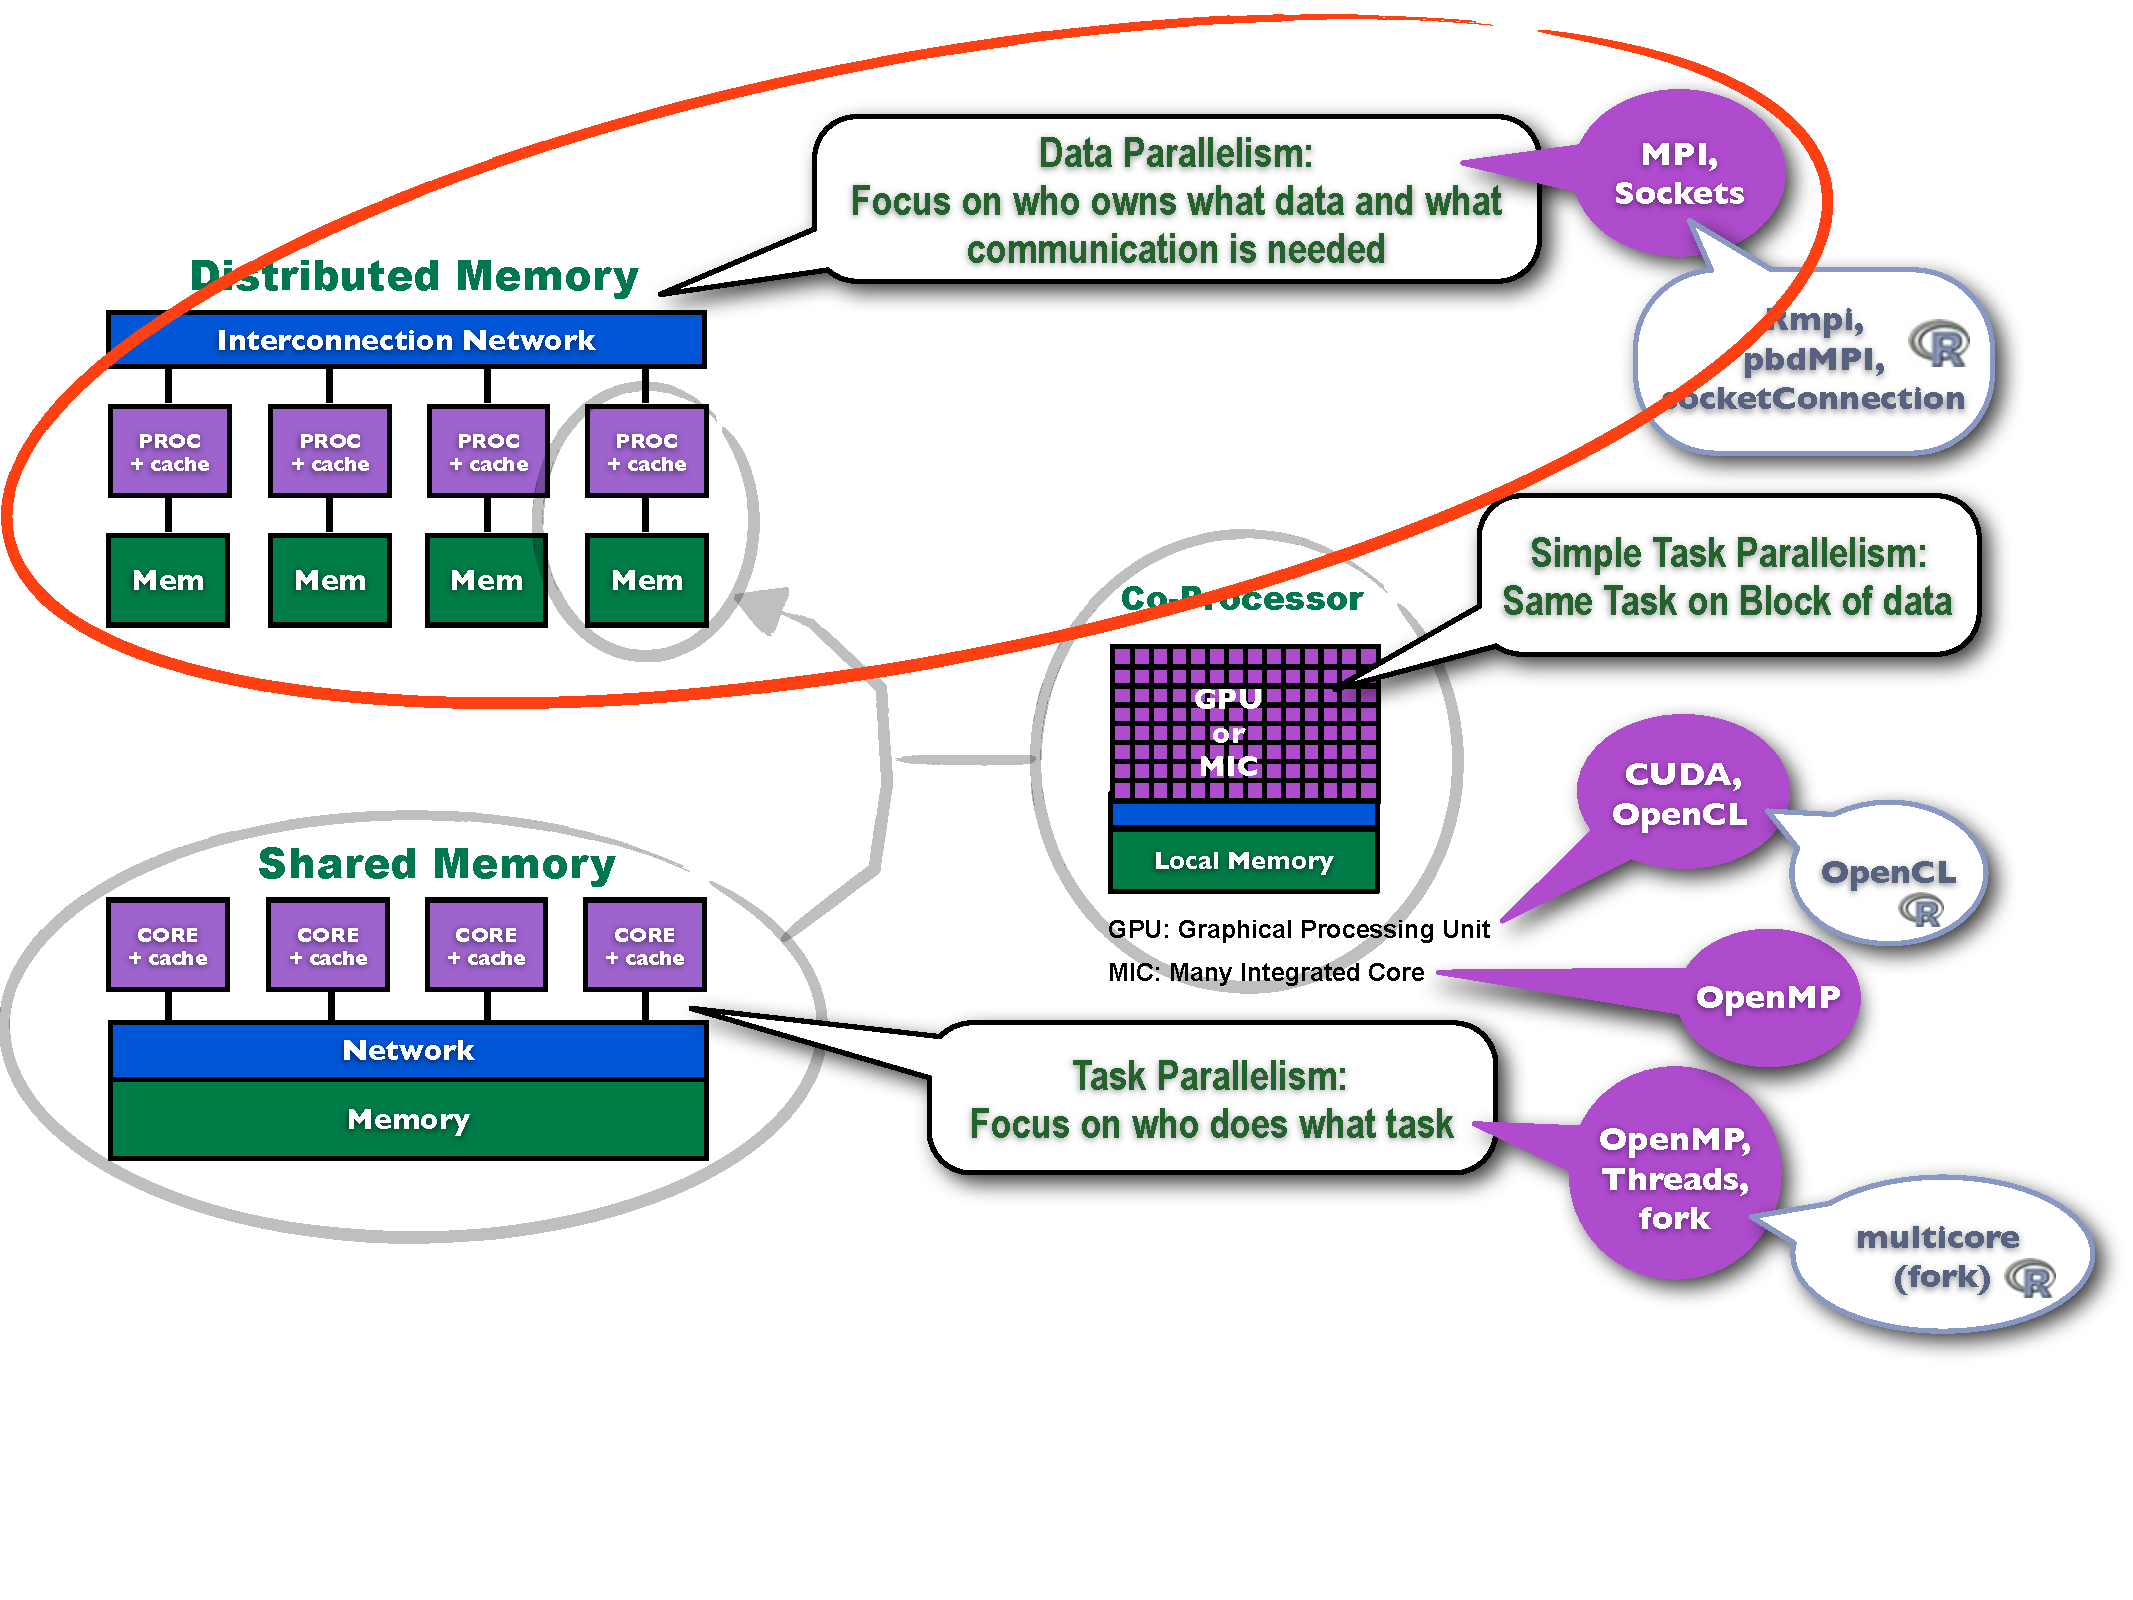
\includegraphics[width=0.95\textwidth]{../common/pics/ParallelHardware8.pdf}
\end{block}
\end{frame}

\begin{frame}
\begin{block}{Last 10 years of Advances}
    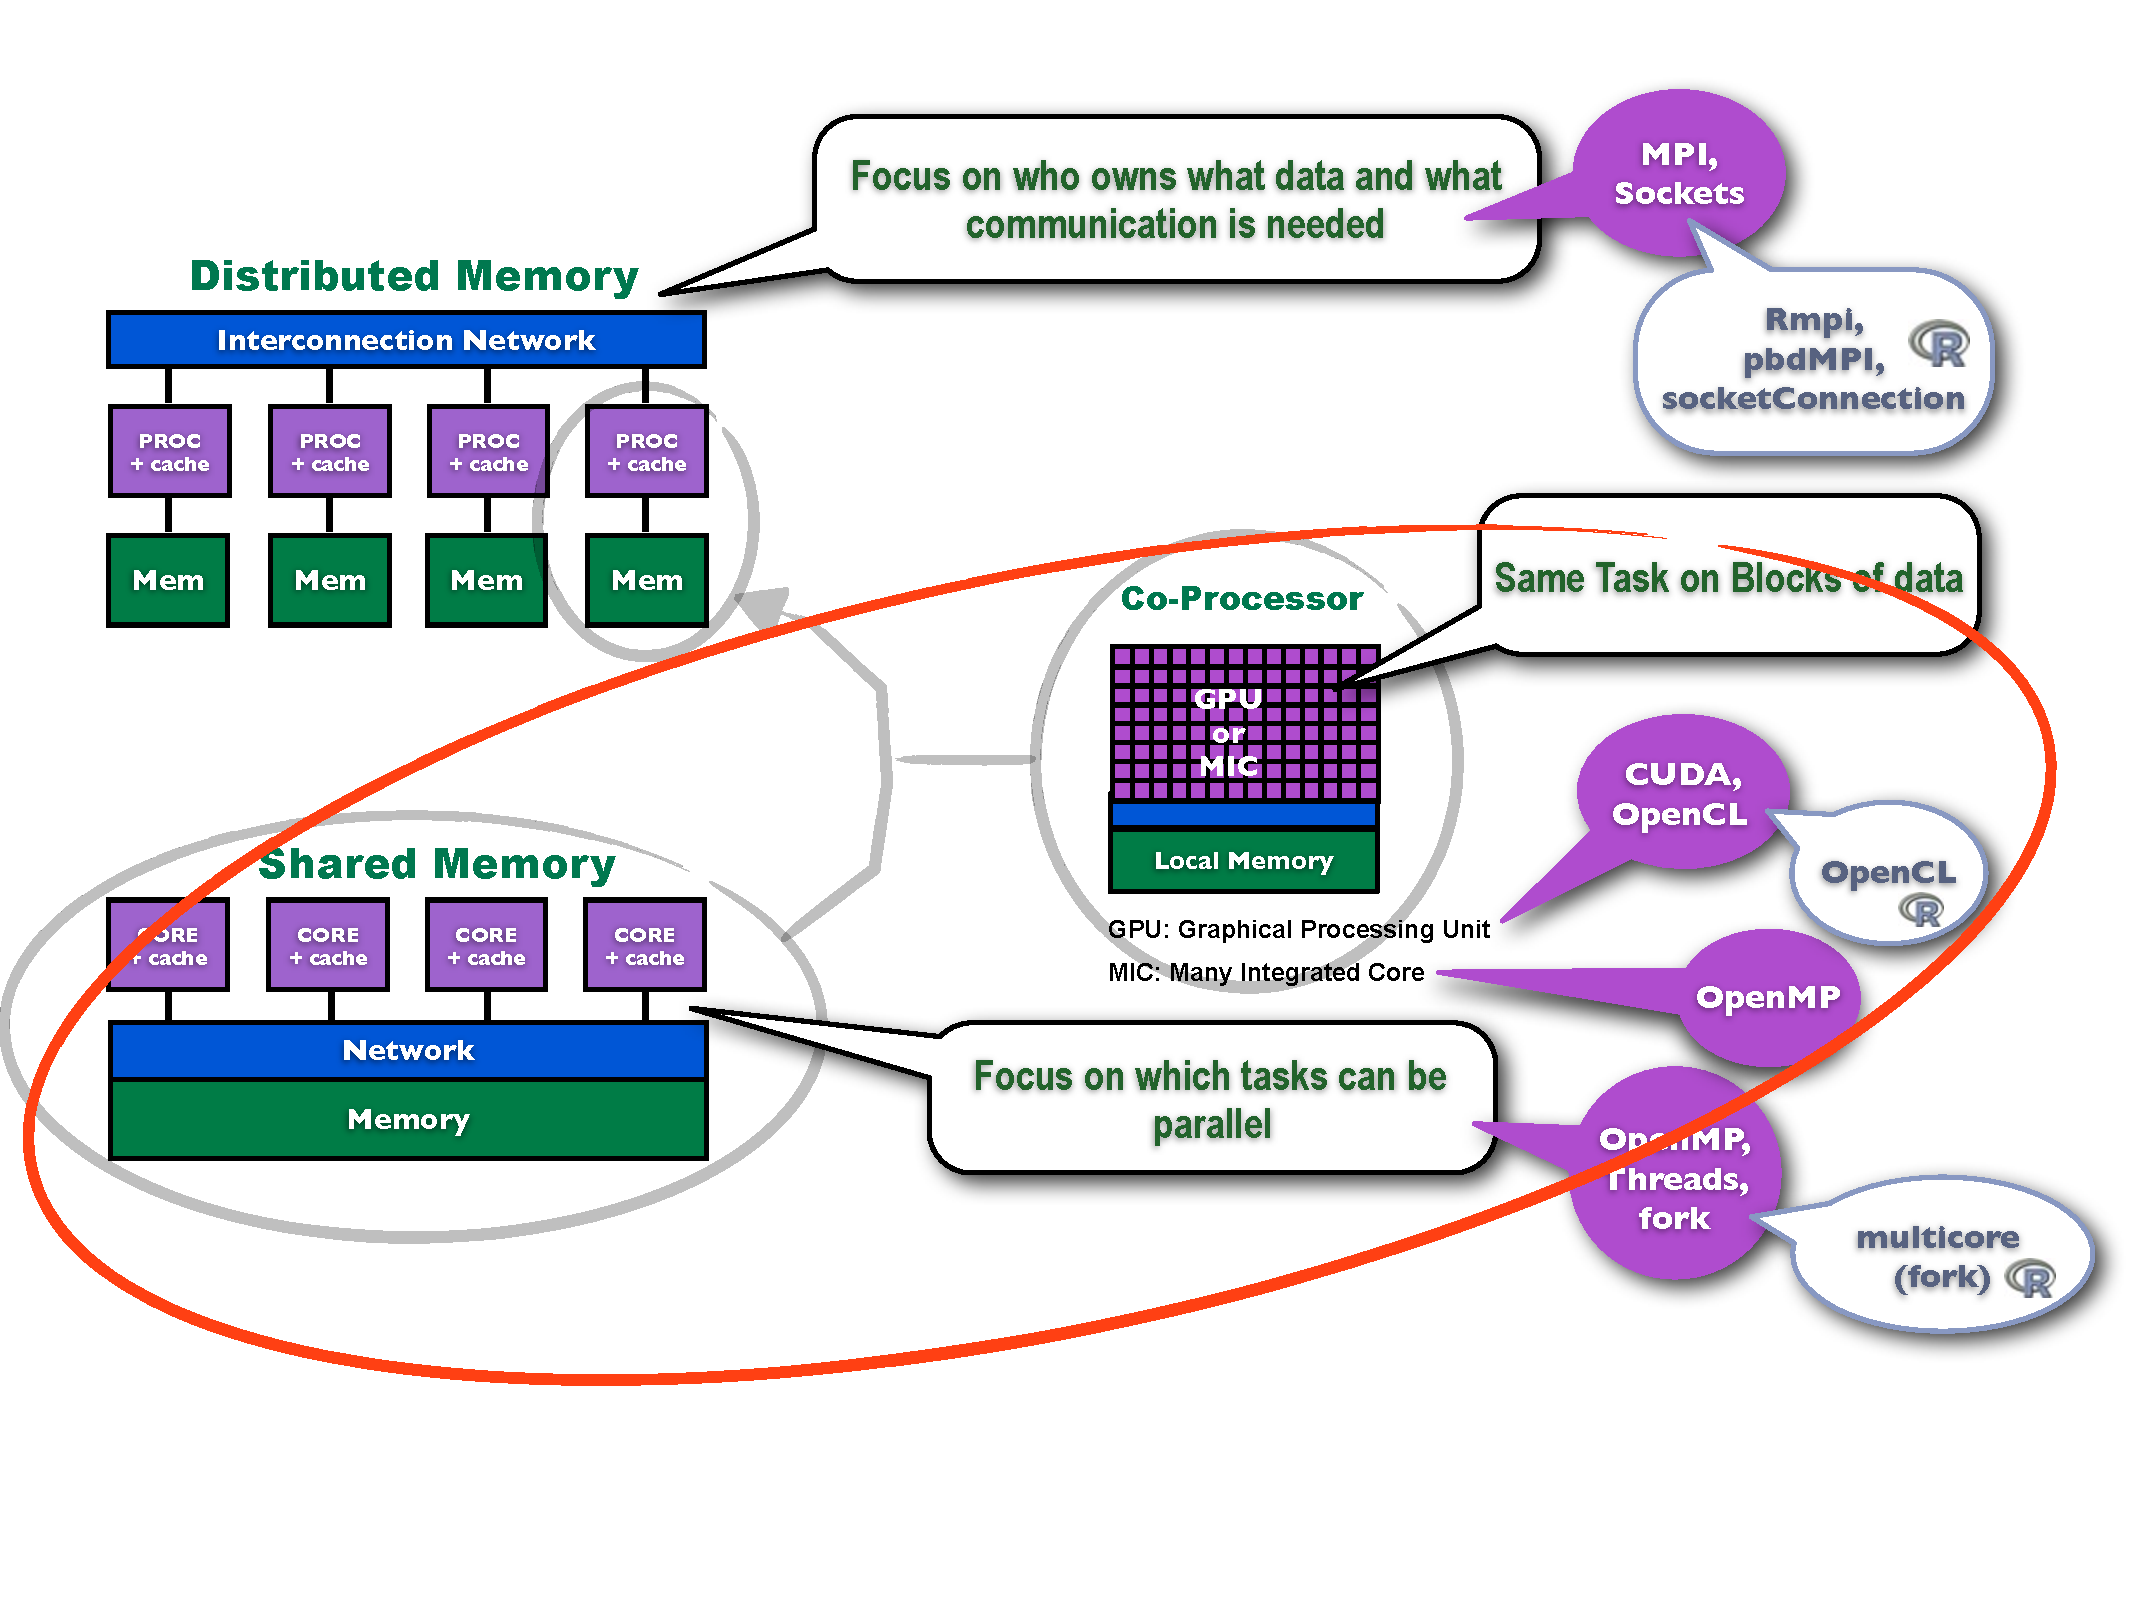
\includegraphics[width=0.95\textwidth]{../common/pics/ParallelHardware9.pdf}
\end{block}
\end{frame}

\begin{frame}
\begin{block}{Putting It All Together Challenge}
    
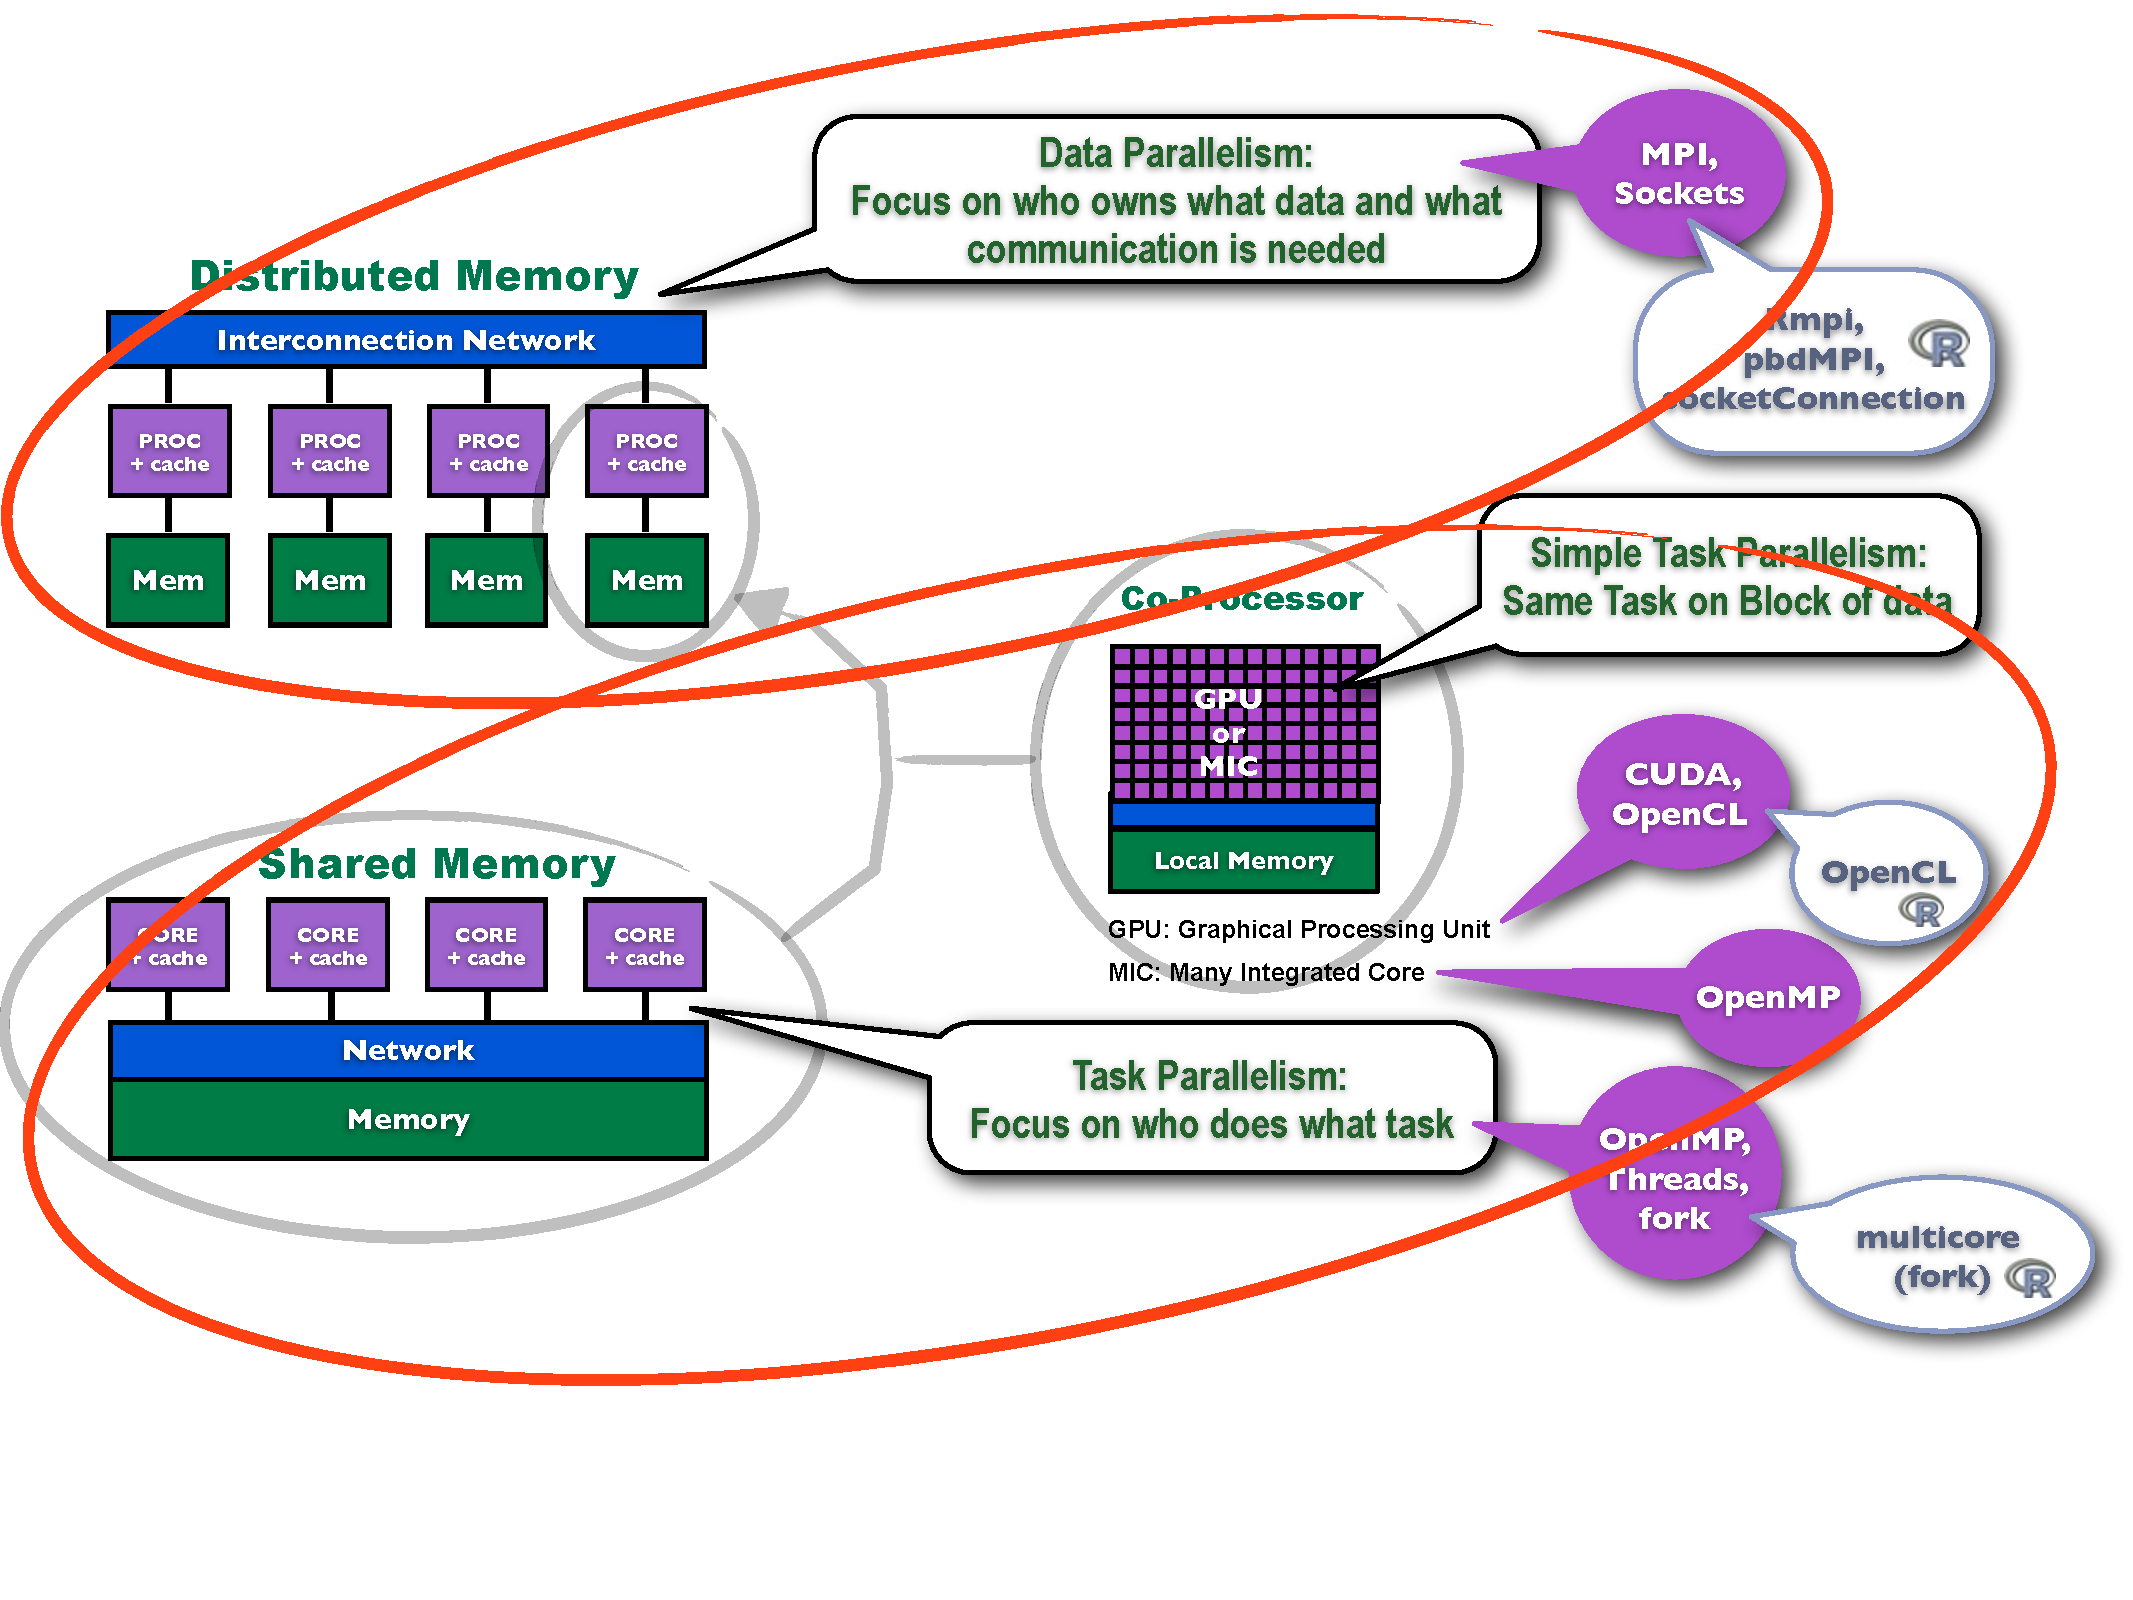
\includegraphics[width=0.95\textwidth]{../common/pics/ParallelHardware10.pdf}
\end{block}
\end{frame}

\begin{frame}
\begin{block}{pbdR Focus on Data Parallelism}
    
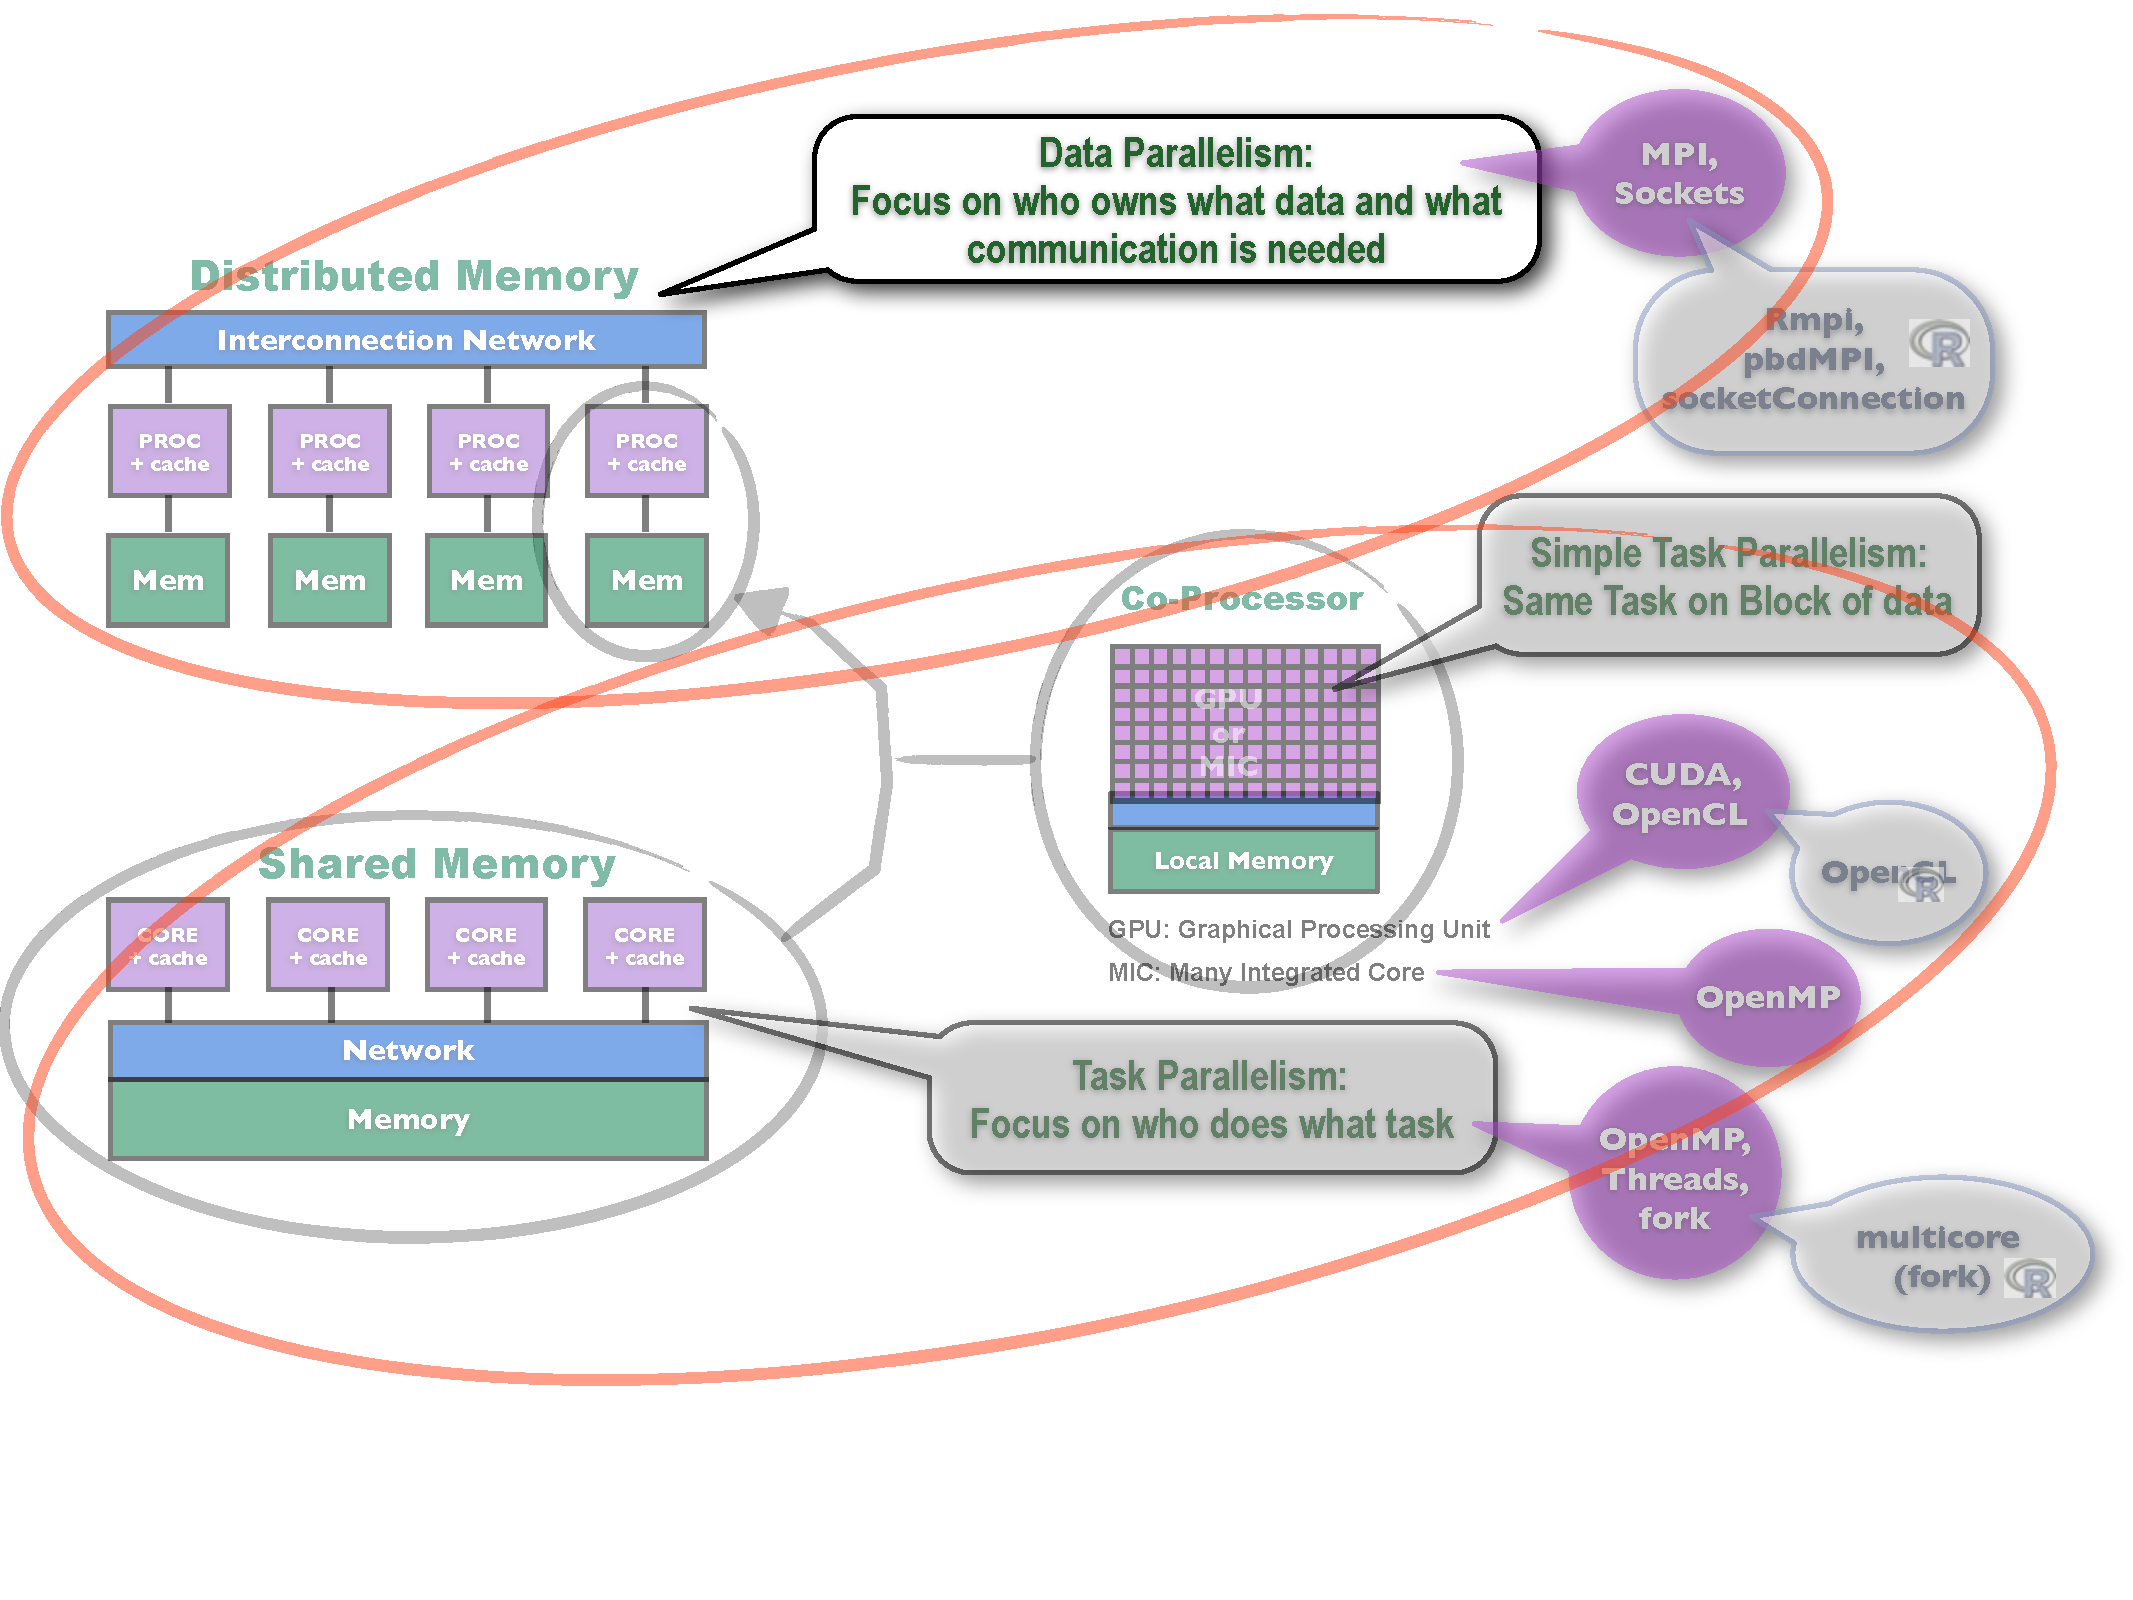
\includegraphics[width=0.95\textwidth]{../common/pics/ParallelHardware11.pdf}
\end{block}
\end{frame}
